%!TEX program = pdflatex
%
%  $Description: INESC ID
%
%  $Author: Dario Nascimento $
%  $Date: 7 Mar 2013
%  $Revision: 1 $
%
%%%%%% ACM %%%%
%\documentclass[preprint,10pt]{sigplanconf}
% preprint      Remove this option only once the paper is in final form.
% 10pt          To set in 10-point type instead of 9-point.
% authoryear    To obtain author/year citation style instead of numeric.
%%%%%% ACM END %%%%

%\documentclass[10pt, conference]{IEEEtran}
\documentclass[10pt,conference]{IEEEtran}

\addtolength{\topmargin}{-2mm}
\addtolength{\topskip}{-2mm}
\addtolength{\textheight}{+5mm}
\addtolength{\textwidth}{+2mm}
\addtolength{\textfloatsep}{-3mm}
\addtolength{\columnsep}{-1mm}
\addtolength{\topsep}{-1mm}
\addtolength{\textfloatsep}{-3mm}



\usepackage{amsmath}

\usepackage[english]{babel}
\usepackage[utf8]{inputenc}
%\usepackage{aeguill}
\usepackage{multirow}
\pagestyle{empty}
\usepackage{graphicx}
\usepackage{float}
\usepackage{tabu}
\usepackage{eurosym} %euro symbol
\usepackage{color} %required to highlight
\usepackage{soulutf8} %Highlight for teacher
\usepackage{amsmath} %math symbols
\usepackage[nolist]{acronym}
\usepackage[caption=false,font=footnotesize]{subfig}
\usepackage{sidecap} %caption on side of figure

%-------------------------------------------------------------------------
% correct bad hyphenation here
\hyphenation{op-tical net-works semi-conduc-tor}


%--------------------------------------------------------------------------

\newcommand{\LONG}[1]{}

\begin{document}

%%%%%% ACM
%\special{papersize=8.5in,11in}
%\setlength{\pdfpageheight}{\paperheight}
%\setlength{\pdfpagewidth}{\paperwidth}

% \conferenceinfo{EUROSYS '15}{April 21-24, 2015, Bordeaux, France} 
% \copyrightyear{2015} 
% \copyrightdata{978-1-nnnn-nnnn-n/yy/mm} 
% \doi{nnnnnnn.nnnnnnn}

% Uncomment one of the following two, if you are not going for the traditional copyright transfer agreement.
%\exclusivelicense                % ACM gets exclusive license to publish, you retain copyright
%\permissiontopublish             % ACM gets nonexclusive license to publish (paid open-access papers, short abstracts)
%\titlebanner{banner above paper title}        % These are ignored unless
%\preprintfooter{Shuttle: Intrusion Recovery for PaaS}   % 'preprint' option specified.
%%%%%  ACM END




\title{Shuttle: Intrusion Recovery for PaaS}
%\subtitle{Subtitle Text, if any}
%a%%%% ACM START %%%%%%%%%%
%\authorinfo{}
%\authorinfo{Dario Nascimento, Miguel Correia}
%           {INESC-ID - Instituto Superior Técnico\\Universidade de Lisboa}
%           {dario.nascimento,miguel.p.correia@tecnico.ulisboa.pt}
%%%% ACM end %%%%%%%%
\author{
	\IEEEauthorblockN{Dário Nascimento, Miguel Correia}\\
	\IEEEauthorblockA{INESC-ID, Instituto Superior Técnico, Universidade de Lisboa\\
	%Lisboa, Portugal\\
	\{dario.nascimento,miguel.p.correia\}@tecnico.ulisboa.pt}
	}

\maketitle

%insert page numbers:
\thispagestyle{plain}
\pagestyle{plain}

% For peer review papers, you can put extra information on the cover page as needed:
\ifCLASSOPTIONpeerreview
\begin{center} \bfseries Regular Paper \end{center}
\fi
%
% For peerreview papers, this IEEEtran command inserts a page break and
% creates the second title. It will be ignored for other modes.
\IEEEpeerreviewmaketitle


%!TEX root = ../../tese.tex
%!TEX encoding = UTF-8 Unicode

\begin{acronym}[IHE]
	%\acro{DAG}{\emph{directed acyclic graph}}
	\acro{ACID}{\emph{Atomicity, Consistency, Isolation and Durability}}
	\acro{API}{\emph{Application Programming Interface}}
	\acro{AWS}{\emph{Amazon Web Services}}
	\acro{BDB}{\emph{Berkeley DB}}	
	\acro{CAP}{\emph{Consistency, Availability, Partition Tolerance}}
	\acro{CPU}{\emph{Central Processing Unit}}
	\acro{CRUD}{\emph{create, read, update and delete}}
	\acro{CSP}{\emph{Cloud service providers}}
	\acro{DBMS}{\emph{Database Management System}}
	\acro{DFS}{\emph{Deep First Search}}	
	\acro{DHT}{\emph{Distributed Hashtable}}	
	\acro{DOM}{\emph{Document Object Model}}
	\acro{EBS}{\emph{Elastic Block Store}}
	\acro{EC2}{\emph{Elastic Compute Cloud}}
	\acro{ECU}{\emph{EC2 Compute Unit}}
	\acro{ELB}{\emph{Elastic Load Balancer}}	
	\acro{HTTPS}{\emph{Hypertext Transfer Protocol Secure}}
	\acro{HTTP}{\emph{Hypertext Transfer Protocol}}
	\acro{IaaS}{\emph{Infrastructure as a Service}}
	\acro{IDL}{\emph{Interface Description Language}}
	\acro{IDS}{\emph{Intrusion detection system}}
	\acro{IMAP}{\emph{Internet Message Access Protocol}}
	\acro{IOPS}{\emph{Input/Output Operations Per Second}}	
	\acro{IP}{\emph{Internet Protocol}}
	\acro{JAX-WS}{\emph{Java API for XML Web Services }}
	\acro{JIT}{\emph{Just-in-time}}
	\acro{JVM}{\emph{Java Virtual Machine}}
	\acro{MVC}{\emph{Model View Controller}}
	\acro{NIO}{\emph{Non Blocking IO}}	
	\acro{NIST}{\emph{National Institute of Standards and Technology}}
	\acro{NoSQL}{\emph{Not only SQL}}
	\acro{OWASP}{\emph{Open Web Application Security Project}}	
	\acro{PaaS}{\emph{Platform as a Service}}
	\acro{protobuf}{\emph{Google Protocol Buffers}}	
	\acro{QA}[Q\&A]{\emph{Questions and Answers}}
	\acro{RDBMS}{\emph{Relational Database Management System}}
	\acro{REST}{\emph{Representational State Transfer}}
	\acro{RID}{\emph{Request ID}}	
	\acro{RMI}{\emph{Remote Method Invocation}}	
	\acro{RPC}{\emph{Remote Procedure Call}}	
	\acro{S3}{\emph{Simple Storage Service}}
	\acro{SaaS}{\emph{Software as a Service}}
	\acro{SID}{\emph{Snapshot ID}}	
	\acro{SOAP}{\emph{Simple Object Access Protocol}}	
	\acro{SQL}{\emph{Structured Query Language}}
	\acro{SRD}{\emph{Shuttle Request Data}}
	\acro{SSD}{\emph{Solid State Disk}}
	\acro{SSH}{\emph{Secure Shell}}
	\acro{SSL}{\emph{Secure Socket Layer}}
	\acro{TCP}{\emph{Transmission Control Protocol}}
	\acro{TID}{\emph{Thread Id}}
	\acro{VM}{\emph{Virtual Machine}}
	\acro{VPC}{\emph{Virtual Private Cloud}}	
	\acro{YCSB}{\emph{Yahoo! Cloud Serving Benchmark}}
\end{acronym}

%!TEX root = ../paper.tex
%!TEX encoding = UTF-8 Unicode

\begin{abstract}
The number of applications being deployed using the Platform as a Service (PaaS) cloud computing model is increasing. Despite  the security controls implemented by cloud service providers, we expect intrusions to strike such applications. We present Shuttle, a novel intrusion recovery service. Shuttle recovers from intrusions in applications deployed in PaaS platforms.
%
Our approach allows undoing changes to the state of PaaS applications due to intrusions, without loosing the effect of legitimate operations performed after the intrusions take place. We combine a record-and-replay approach with the elasticity provided by cloud offerings to recover applications deployed on various instances and backed by distributed databases. The service loads a database snapshot taken before the intrusion and replays subsequent requests, as much in parallel as possible, while continuing to execute incoming requests. 
%Shuttle not only avoids application downtime during recovery, but also allows customers to deploy new application versions to fix previous software flaws.
%
We present an experimental evaluation of Shuttle on Amazon Web Services. We show Shuttle can replay 1 million requests in 10 minutes and that it can duplicate the number of requests replayed per second by increasing the number of application servers from 1 to 3. 

%The increasing number of intrusions and critical applications deployed in cloud systems requires an approach to recover from intrusions. We present Shuttle, a novel service \hl{approach?} for \acf{PaaS} systems that gives cloud providers the capability to allow their customers to recover their applications from intrusions. Through exploiting the novel \ac{PaaS} architecture \hl{model?}, the proposed service removes security intrusions due to software flaws or corrupted user requests and supports corrective and preventive maintenance of applications deployed in \ac{PaaS}.

%We combine the record-and-replay approach with the elasticity and pay-per-usage model of \ac{PaaS} to recover from intrusion in applications deployed on various instances and backed by distributed database. We propose to load a previous database snapshot and replay the requests in parallel using a set of cloud instances to reduce the recovery period. Shuttle not only avoids application downtime during the recovery but also allows customers to deploy new application versions to fix previous software flaws.

%Through our evaluation, we demonstrate that Shuttle incurs negligible \hl{acceptable?} performance overhead and that performing parallel replay using \hl{XXX} client instances and \hl{XXX} new application instances and \hl{XXX} database instances can reduce the recovery period by \hl{XXX}\%. We also show Shuttle can recover an application with \hl{XXX} requests, storing \hl{XXX} of metadata and replaying the requests in \hl{xxx} seconds using \hl{xxx} cloud instances.

\end{abstract}

%%!TEX root = ../paper.tex
%!TEX encoding = UTF-8 Unicode

%\category{CR-number}{subcategory}{third-level}

\keywords Intrusion Recovery, Replay, Cloud Computing, Platform as a Service

%\keywords Intrusion Recovery, Intrusion Tolerance, Survivability, Replay, Cloud Computing, Platform as a Service, Distributed Database Systems
%\begin{IEEEkeywords}
%	Intrusion Recovery; Replay; Cloud Computing; Platform as a Service;
%\end{IEEEkeywords}
%!TEX root = ../tese.tex
%!TEX encoding = UTF-8 Unicode
\chapter{Introduction}\label{chapter:introduction}
%What is PaaS?
\ac{PaaS} is a cloud computing model that supports automated configuration and deployment of applications \cite{Vaquero2008,Vaquero2011,Armbrust,Mell}. While the \ac{IaaS} model is being much used to obtain computation resources and services on demand \cite{Lenk2009,Armbrust}, \ac{PaaS} aims to reduce the cost of software deployment and maintenance abstracting the underlying infrastructure. The model defines a well tested and integrated environment in which clients (\textit{tenants}) design, implement, deploy and run their applications on a managed cloud infrastructure through a set of middleware services. Examples of these services are load-balancing, automatic server configuration and storage. These services are paid-per-usage and turn the application easy to deploy and scale.
\ac{PaaS} platforms are provided either by cloud providers, such as Windows Azure \cite{azure}, Google App Engine \cite{GoogleAppEngine}, Heroku \cite{Heroku}, Openshift \cite{OpenShift} and Amazon Elastic Beanstalk \cite{AmazonElasticBeanstalk}, or by open source projects \cite{Appscale,Cloudfoundry,ApacheStratos}. Besides natural metrics such as cost and performance, the success of \ac{PaaS} systems will also be established by their features, for instance capability to recover from intrusions.


\section{Problem Statement}\label{sec:introduction:problem}
%Intrusions happening more and more
The number of applications running in cloud computing platforms, including those based on the \ac{PaaS} model, is increasing rapidly. 
Many of these applications are critical for their companies and contain valuable information, so the exploitation of vulnerabilities is attractive and profitable. Consequently, the risk of intrusion is high. An intrusion happens when an attacker exploits a vulnerability successfully. Intrusions are considered faults. Faults may cause system failure and, consequently, application downtime and significant business losses \cite{Patterson2002a}. The recent case of the cloud-based Code Spaces service is conspicuous: hackers deleted most of its data and backups, leading to the termination of the service \cite{McAllister:14}. 

%Problems  
\ac{CSP} implement several security controls. Most of these controls aim to prevent and detect intrusions: access control, firewalls, intrusion detection and prevention systems, network access control, vulnerability scanning, etc. Despite the importance of these mechanisms, applications often contain design or configuration vulnerabilities that let intrusions happen \cite{Williams2013,Hubbard2010}. Complexity and budget/time constraints \cite{Charette2005}, weak users passwords or bad security policies are known causes of these problems. The recent case of the bash bug (or Shellshock) shows that there are other reasons such as legacy software being used in ways that were unpredictable when it was developed \cite{Sidhpurwala:14}. Attackers can spend years developing new ingenious and unanticipated attack methods having access to what protects the application. On the opposite side, guardians have to predict new methods to mitigate vulnerabilities and to solve attacks in few minutes to prevent intrusions.

%Fault tolerance does not work
Much research has been done on mechanisms to tolerate Byzantine faults, including intrusions \cite{Castro2002,Verissimo2003,Gupta:03}. However, most of these techniques do not prevent application level attacks or user mistakes. For instance, if attackers steal legitimate user credentials, they are able to modify the state of the applications violating their security policy. In summary, there are several paths for intrusions to happen, even if mechanisms to prevent or tolerate them are used.\\ %Therefore, the application integrity can be compromised and the intrusion reaches its goal bringing the system down to repair. \\

%Manual recovery is error prone
We assume intrusions can happen and their effects need to be removed from the applications' state. This removal is often done manually by system administrators. Administrators have to detect the intrusion, understand the parts of the state compromised directly by the intrusion or contaminated by operations that used compromised state, and clean the state manually. For instance, most of full-backup solutions revert the intrusion effects but require extensive system administrator effort to restore the effect of the legitimate actions. This process is error-prone, often takes long and causes application downtime \cite{Brown2001}. Intrusion recovery systems aim to automate these steps and mitigate these issues.

%what is the problem of related works?
Previous intrusion recovery systems targeted operating systems \cite{taser,retro}, databases \cite{itdb,phoenix}, web applications \cite{goel,warp,aire} and other services \cite{undoForOperators}. Yet, none of them was designed for cloud applications, which are often deployed in multiple servers and use background databases. Furthermore, most cause downtime, which is undesirable in online services.
 
\section{Goals and Main Contributions}\label{sec:introduction:goals}
%Recovery in Cloud
The primary goal of this thesis is to design, develop and evaluate a system to recover from intrusions in cloud computing. In particular, the system shall allow tenants to keep their \ac{PaaS} applications operational despite intrusions. The idea is to accept intrusions can happen, thus to provide a system to remove their effects from the application's state and restore the state's integrity. 

%Recovery instead of preventing
The approach followed in this dissertation consists in recovering the applications state when intrusions happen, instead of trying to prevent them from happening. Intrusion recovery systems do not aim to substitute prevention but to be an additional security mechanism. Similarly to fault tolerance, we accept that faults occur and have to be processed. However, we aim to decrease the applications' Mean Time to Repair (MTTR), not the Mean Time to Failure (MTTF). Doing so, we expect to increase the applications' availability, which is given by $Availability=MTTF/(MTTF+MTTR)$. \\

%Recovery in PaaS using a service: goals of the contribution
The main contribution of this dissertation is a novel \emph{intrusion recovery service} for \ac{PaaS} systems, named \emph{Shuttle}. Shuttle is a service that aims to make \ac{PaaS} applications operational despite intrusions, helping tenants to recover their applications from software flaws and malicious, or accidental, corrupted user requests without requiring application downtime during the process. When an intrusion is detected, tenants can use this service, which is offered by the \ac{CSP}, to remove intrusions' effects and recover the integrity of their applications. In this dissertation, we are concerned with the applications' availability and the integrity of their state, not their confidentiality. Consequently, the proposed service does not aim to deal with information leaks.



%How it works summary
Shuttle assumes a client-server model in which clients communicate with the servers in the cloud using \ac{HTTP}/\ac{HTTPS} or protocols encapsulated on top of them (e.g., \acs{SOAP}, \acs{REST}). For each application deployed in the \ac{PaaS} system, Shuttle records the requests issued by clients and creates periodic snapshots of the application database. 

After detection of the intrusion, Shuttle loads the snapshot that precedes the beginning of the intrusion and replays only the legitimate requests to recreate an intrusion-free application state. Requests are replayed asynchronously and, whenever possible, concurrently. Even so, the recovery process is deterministic because operations to each data item must have the same order as on first execution. 

Dependencies established at database level during the requests' first execution are used to create independent clusters of requests that can be replayed concurrently. We propose a branching mechanism to maintain the service available continuing to execute incoming requests while replaying the requests. 

We introduce a novel approach to remove the intrusion effects in which the \ac{PaaS} controller terminates the current application instances, launches new instances and deploys an updated software version, which may fix previous flaws.



%why PaaS?
Unlike previous intrusion recovery systems, Shuttle is provided as a service to developers and tenants of \ac{PaaS} applications. Consequently, it can be well tested and available without depending on being correctly setup by the application developers. We also leverage the elasticity of \ac{PaaS} infrastructures to reduce the service costs and the recovery period. Specifically, Shuttle is designed to allocate more servers during the recovery period to accommodate the throughput of requests being replayed, and release them at the end, with a proportional impact on service costs. The decline in computation and storage costs in public cloud providers makes affordable to store user requests, to use database snapshots and to replay previous user requests.

%Contributions
We propose, to the best of our knowledge, the first intrusion recovery service for \ac{PaaS} applications. The main contributions of this dissertation are the following:
\begin{itemize}
\item a new intrusion recovery approach provided as a service integrated in a \ac{PaaS} system and taking into consideration applications running in various instances backed by distributed databases;
\item a method to order the replayed user requests considering their accesses to databases;
\item accomplishing intrusion recovery without service downtime using a branching mechanism;
\item leveraging the resource elasticity and pay-per-use model in \ac{PaaS} environments to record and launch multiple clients to replay previous non-malicious user requests as concurrently as possible to reduce the recovery time and costs;
\item a mechanism to do a globally transaction-consistent snapshot of \acs{NoSQL} databases;
\item an approach to remove intrusions redeploying the applications;
\end{itemize}

\section{Thesis Structure}\label{sec:introduction:structure}
This document is structured as follows. In Chapter \ref{chapter:related_work}, we present the fundamental concepts and previous intrusion recovery proposals. In Chapter \ref{chapter:architecture}, we describe the architecture of \ac{PaaS} systems and the proposed mechanism for intrusion recovery service. In Chapter \ref{chapter:implementation}, we describe the platform and components of the prototype of Shuttle. The work is evaluated in Chapter \ref{chapter:evaluation} and concluded in Chapter \ref{chapter:conclusion}.
%!TEX root = ../paper.tex
%!TEX encoding = UTF-8 Unicode

\section{Background and Related Work}\label{sec:background}
%Como e que as apliccaoes sao recuperadas, de modo generico e com o related work incluido
%and Related Work

This section formalizes several approaches to perform intrusion recovery and presents the main related work. 
%
An application execution is modeled as a set of actions $A$ on a set of objects $D$. Actions are described by operations (read, write, others more complex), the value(s) read/written, and a timestamp (which defines the order of the actions). Each object has a state (or value) and a set of operations that can modify it. We define $A_{intrusion}$ as the subset of actions of $A$ whereby the attacker compromises the application during the intrusion, $A_{after}$ as the subset of actions that began after the intrusion began (including the first action of the intrusion), and $A_{legal}$ as the subset of legitimate actions in $A$, i.e., $A_{legal} = A \backslash A_{intrusion}$.

Intrusion recovery services aim to remove the effects of malicious actions setting the application state to a state set only by legitimate actions. 
%The recovered application state shall respect the application specification (correctness) \cite{Aviz}.
%
A \textit{backup} mechanism is a basic recovery service that can set objects to the state they had before an intrusion began. The new state excludes the effects of the attacker's actions, but also the effects of any legitimate actions performed after the backup was done. This second aspect is undesirable, so recent intrusion recovery systems aim to avoid it.
%
This is the case in the closest works to ours: Aire \cite{aire}, Warp \cite{warp}, Goel \cite{Akkus2010}, and Undo for Operators (UO) \cite{undoForOperators}. None of these works handles recovery in cloud environments.

An action is considered \textit{tainted} at a certain instant if it is one of the attacker's malicious actions or if it reads an object written by a tainted action (called a \textit{tainted object}). Since actions are contaminated by malicious actions through objects, to remove the state written by tainted actions it is necessary but not sufficient to obtain the state produced by the legitimate actions. 

%mpc: comentei pois nao percebi a mensagem que queriamos passar e nao parece exacto
%Some intrusion recovery systems \cite{taser,itdb,phoenix} attempt to do it \textit{replacing} the value of the tainted objects by a previous value. These systems keep the objects written by legitimate actions unmodified. %rever o taser, itdb e phoenix para confirmar


%mpc: juntei 2 paragrafos e limpei as varias repeticoes das mesmas ideias
Consider a hypothetical application execution. At a certain point in time after an intrusion, the application is stopped and the sequence of actions executed ($A$) is purged of the actions in $A_{intrusion}$.
% i.e., the intrusion actions $A_{intrusion}$ are not executed. 
%
Then, the state is rewind to the beginning of the application execution and only the actions in $A_{recovered} = A \backslash A_{intrusion} = A_{legal}$ are re-executed. That re-execution is intrusion-free as 
%mpc: D_intrustin e D_tainted nem sequer foram definidos
%$A \cap A_{intrusion} = \emptyset \implies D_{intrusion} = \emptyset, A_{tainted} = \emptyset \implies D_{tainted} = \emptyset$. 
$A \cap A_{intrusion} = \emptyset \implies A_{tainted} = \emptyset$. 
%Since the malicious actions were removed, the state, $D$, would not have values imposed by $A_{intrusion}$. 
%For this reason, the sequence of tainted actions $A_{tainted}$ would be empty. 
The set of tainted actions of the first execution that are not in $A_{intrusion}$ are re-executed but read different values (not imposed by the attacker) and have a different execution. 
%Therefore, if $A_{intrusion}$ and $D_{intrusion}$ are removed, then $A_{tainted}$ should be \emph{replayed} because the actions of $A_{tainted}$ are not contaminated by malicious data during their re-execution. 
The replay process restores the application to a correct state $D_{recovered}$, which is not compromised by the intrusion.

That generic approach is unfeasible without the use of snapshots.
The sequence of actions performed before the intrusion $A_{before} = A \backslash A_{after}$ can be long and each action takes non-null time to execute, so replaying $A_{before}$ may be unfeasible. Moreover, a log of all the actions executed may be too large.
We define the subsets $D_{snapshot}(t)$ and $A_{snapshot}(t) : A_{snapshot}(t) \subset A$ as the subsets of objects and actions executed before the begin of a snapshot operation at instant \textit{t}. 
%The snapshot operation copies the value of the object immediately or on the next write operation. 
If the intrusion happens after $t$, then $A_{after} \cap A_{snapshot}(t) = \emptyset \implies (A_{intrusion} \cup A_{tainted}) \cap A_{snapshot}(t) = \emptyset$, i.e., the snapshot is not affected by the intrusion. For that reason, the service can replay only $A \backslash A_{snapshot}(t) \backslash A_{intrusion}$ using the object set $D_{snapshot}$ as base. 

There are two distinct replay approaches to update the set of object $D$ to $D_{recovered}$, 
%because of changes in the execution of $A_{tainted}$
selective replay and full replay. 
A \textit{version} is a snapshot of a single object value at an instant $t$. Versions can be recorded with the sequence of actions that write the objects before the instant $t$.
The \textit{selective replay} approach loads only the versions of the tainted objects, $D_{tainted}$, previous to the intrusion, instead of loading a previous version of every object \cite{taser,warp,Akkus2010}. Then, it replays only the legitimate actions, which were tainted, $A_{tainted} \backslash A_{intrusion}$, to update the objects in $D$. The state of the objects in $D_{legal} \backslash D_{tainted}$ remains unmodified. 
The other approach, \textit{full replay} \cite{undoForOperators}, loads a snapshot previous to the intrusion moment and replays every action in $A \backslash A_{snapshot}(t) \backslash A_{intrusion}$. This approach is slightly simpler than the other, but in general takes longer to execute. 

%mpc: movi a definicao de version para o parag anterior porque fazia la' falta
%A version is a snapshot of a single object value before the instant t. They can be recorded with the sequence of actions that read or write them before the instant t. We define a compensating action as an action that reverts the effects of a original action, for instance writing a previous value. A compensation process can obtain a previous snapshot or version. For this propose, we define the sequence Acompensation(t) as the compensation of Aposteriori(t), the sequence of actions after instant t. The compensation process applies the sequence of compensating actions Acompensation(t) on the current version of the objects, in reverse order, to obtain a previous snapshot or version.


\LONG{

%\hl{o proximo paragrafo resume todo o processo de replay mas acho que poderia ser tirado porque vai sendo explicado ao longo do paper}  %mpc: de facto e' repetido logo no inicio da seccao seguinte
Recovery services have two distinct phases: record and recovery. The \emph{record phase} is the service usual state where the application is running and the service records the application actions. In order to perform replay, the application actions do not need to be idempotent but their re-execution must be deterministic (given the same initial state they produce the same final state). The record phase should record the actions input and the value of every non-deterministic behavior to turn their re-execution into a deterministic process. The \emph{recovery phase} can be subdivided in three: determining the affected actions and/or objects, removing these effects, and replaying the actions necessary to recover a consistent state. In this paper we present a recovery service that supports \textit{runtime recovery}, i.e., that allows the record and recovery phases to occur simultaneously.

}

\LONG{

\hl{este explica o dependency graph. ou o related work sai e vem para aqui ou entao nao vale a pena ter um pagrafo a falar disto quando ha uma seccao} %mpc: ok, comentei
Most intrusion recovery services record both the actions and  the objects they accessed  \cite{Akkus2010,itdb,warp}. Since the actions read and write objects from a shared set of objects $D$, we can establish dependencies between actions. Dependencies can be seen as an \textit{action dependency graph} or an \textit{object dependency graph}. The nodes of an action dependency graph represent actions and the edges indicate dependencies though shared objects. An object dependency graph establishes dependencies between objects through actions. Dependency graphs have been used to order the re-execution of actions \cite{undoForOperators}, get the sequence of actions affected by an object value change \cite{warp}, get the sequence of actions tainted by an intrusion \cite{Akkus2010} or resolve the set of objects and actions that caused the intrusion using a set of known tainted objects \cite{backtracker}. 

%A \textit{taint algorithm} aims to define the tainted objects $D_{tainted}$ from a set of malicious actions $A_{intrusion}$ or objects $D_{intrusion}$ using a dependency graph. This method is used by selective replay approaches. The \textit{taint propagation via replay} \cite{retro} algorithm begins with the set $D_{tainted}$ determined by the base taint algorithm \hl{o que significa?} and expands the set \hl{o que significa?} $D_{tainted}$. It is used to restore the values of $D_{intrusion} \cup D_{tainted}$ and to replay only the legal actions that output $D_{intrusion} \cup D_{tainted}$ during the original execution. Then it replays the actions dependent from $D_{intrusion} \cup D_{tainted}$, updating their output objects. While the forward actions have different input, they are also replayed and their outputs are updated. 

Dependencies are established during the record phase or at recovery time using the objects and actions. The level of abstraction influences the record technique and the dependency extraction method. The abstraction level defines the recoverable intrusions: operating system \cite{taser,retro}, database \cite{itdb,phoenix}, and application \cite{Akkus2010,warp,aire}. In the next sections, we present Shuttle, an intrusion recovery service which recovers from intrusions using the dependencies established at database and application level.

}

%!TEX root = ../tese.tex
%!TEX encoding = UTF-8 Unicode

\chapter{The Shuttle Architecture}
\label{chapter:architecture}
This chapter describes the overall system architecture of Shuttle and outlines its central functional components. The main design goal is to help \ac{CSP} customers to recover from intrusions in their applications deployed in \ac{PaaS}. We consider three actors: the \ac{CSP}, which provides the platform, the \emph{tenants}, who deploy their applications in the platform, and the \emph{users}, who access the applications. Shuttle is a service designed to be offered by a \ac{CSP}.

We introduce the main requirements in Section \ref{sec:arch:requirements} and describe a generic \ac{PaaS} architecture in Section \ref{sec:arch:paas}. The remaining sections describe the architecture of Shuttle and discuss the main design choices.

\section{Requirements}
\label{sec:arch:requirements}
This thesis addresses the problem of providing an intrusion recovery service for applications deployed in \ac{PaaS}. Our overall goal is to \textit{make \ac{PaaS} applications operational despite intrusions}. More precisely, we aim to create a service, named Shuttle, to help \ac{PaaS} tenants to recover from the following problems in their applications:
\begin{itemize}
\item \textit{Software vulnerabilities:} non-authorized users compromise state by exploiting software vulnerabilities that allow invalid requests to be executed.
\item \textit{Malicious or accidentally corrupted requests:} users, authorized or not, compromise the application state accidentally or intentionally issuing valid requests.
\end{itemize} 




%attack example
For instance, two common attacks that can be used to compromise application state consist in: (1) attackers stealing valid users' credentials and using them to access their data; and (2) doing a \ac{SQL} Injection attack by mixing \ac{SQL} meta-characters with normal input and doing otherwise invalid queries to the database. Both attacks can be performed using apparently valid requests. Consequently, many prevention mechanisms fail to block them.

In order to achieve the above goals, the service shall meet the following requirements: 
\begin{itemize}
\item \textit{Remove intrusion effects:} Remove corrupted data at file system, database and application levels in the application containers and update affected legitimate actions. 
\item \textit{Remove selected malicious actions:} Help tenant to track the intrusion producing the set of actions affected by an externally provided list of malicious actions.
\item \textit{Support software update:} After recovery, the application state has to be compliant with the new version of the software.
\item \textit{Recover without stopping the application:} Recover the application without exposing users to application downtime.
\item \textit{Determinism:} Despite concurrent re-execution of requests, the result of re-execution is the same as the result of first execution if the application source code and requests remain equal.
\item \textit{Low runtime overhead:} The recording of operations or state for recovery purposes should have a negligible impact in the runtime performance.
\item \textit{\acs{NoSQL} database snapshot:} \acs{NoSQL} databases will have to be extended to support database snapshots, in order to reduce the recovery time.
\item \textit{\ac{PaaS} integration:} The source code of the application shall remains unmodified as much as possible. \ac{PaaS} developers do not need to install or configure Shuttle. Shuttle is built in a generic manner and it is reused in each deployed application.
\end{itemize}

Shuttle shall \textit{support software updates} to prevent future intrusions and allow operators to try new configurations or software versions without effects in the application behavior perceived by users. 


\section{Platform as a Service}
\label{sec:arch:paas}
\ac{PaaS} is a cloud computing model for automated configuration and deployment of applications in a cloud infrastructure \cite{Vaquero2008,Vaquero2011,Armbrust,Mell}. \ac{PaaS} enables developers to develop and deploy web applications into production fast by abstracting many details of the underlying infrastructure. Developers access the infrastructure resources, such as storage, through a set of services. These services are often pay-per-usage. \ac{PaaS} provides a deployment environment for a set of languages. 

%Bottom-layer: IaaS, VMs
Applications are deployed in one or more application servers, e.g., Tomcat or NodeJS. \emph{Containers} \cite{Lenk2009} hold these application servers and provide the required isolation level between the various applications. The word container is often used to refer to lightweight in-kernel resource (CPU, memory and device) accounting, allocation and isolation mechanisms like the \textit{Linux control groups} \cite{Menage2007}. These mechanisms isolate the process, network and file system used by applications that share the same operating system. They can run either directly on the host operating system or in a virtual machine. In this document, we use the word \textit{container or instance} to mean an isolated deployment unit that can be allocated from a resource pool by an orchestration engine. The deployment unit is created using an image and has storage attached. Therefore, our concept of container includes not only \textit{Linux control groups} like systems but also bare metal servers and guest operating systems running on top of hyper-visors, e.g., Xen \cite{xen}, KVM \cite{kvm}. Containers are managed directly or through an orchestration or IaaS system (e.g., OpenStack \cite{openstack}, \ac{AWS} \ac{EC2} \cite{aws}, Eucalyptus \cite{eucalyptus}, Omega \cite{omega}). Containers have one or more associated storage. When the container loads up, it loads an image onto its storage. The image contains, at least, the operating system and the \ac{PaaS} system in order to deploy the application in the container. 

%Components
In order to let Shuttle as generic as possible, we consider the following components of a minimal \ac{PaaS} architecture (Figure \ref{fig:paasArchitecture}):
\begin{itemize}
\item \textbf{Load balancer:} Routes user requests based on application location and container load.
\item \textbf{Instance controller:} Collects the container metering data and performs the configuration, tear-up and tear-down of containers in the instance.
\item \textbf{Cloud controller:} Manages the tear-up and tear-down of containers.
\item \textbf{Metering and billing}: Retrieves the metering data from each container. The load balancer uses this information to perform request routing while the cloud controller automatically decides when to scale.
\item \textbf{Containers:} The isolated environment where applications run.
\item \textbf{Cloud Instances:} The guest operating systems or bare-metal machine where the containers run.
\item \textbf{Authentication manager:} Provides user and system authentication.
\item \textbf{Database instance:} A single \ac{DBMS} shared, or not, between multiple applications. Most database middleware are built-on multiple containers to provide scalability and replication.
\item \textbf{Authentication manager:} Provides user and system authentication.
\end{itemize}

\begin{figure}
\centering
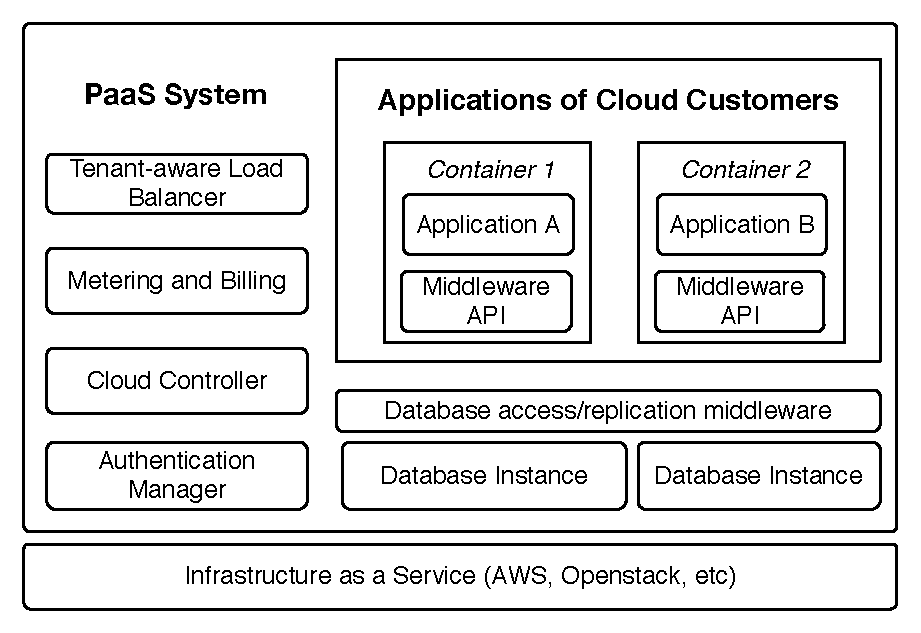
\includegraphics[width=100mm]{images/paas}
\caption{Generic \ac{PaaS} architecture}
\label{fig:paasArchitecture}
\end{figure}

\ac{CSP} also deploy the database management systems in containers. Their data is accessed as a service by the developers. Most of the applications deployed in \ac{PaaS} are designed to scale horizontally, i.e., to scale adding more containers. Therefore, the database and/or the session cookies often maintain the application state. The \ac{PaaS} systems are often integrated with code repositories and software development tools reducing the time deploy of applications in cloud environments. Users may access the website connecting to the load balancer via \ac{HTTPS}, which will decrypt the \ac{SSL} session and forward the unencrypted requests to application containers. As the traffic increases, the load balancer may become a performance bottleneck if the system does not provide enough resources to handle the user traffic.\\

We assume applications to store their persistent state only in databases. Shuttle's architecture can be extended to encompass object storage, for instance \ac{AWS} \ac{S3}. We do not consider a possible state stored in the filesystem because \ac{PaaS} applications are supposed to be scalable, thus the instances file system is frequently destroyed.

%%%%%%%%%%%%%%%%%%%%%%%%%%%%%%%%%%%%%%%%%%%%%%%%%%%%%%%%%%%%%%%%%%%%%%%%%%%%%%%%%%%%%%%%%%%
\FloatBarrier
\section{Shuttle Overview}
\label{sec:arch:overview}
Shuttle is an intrusion recovery service for \ac{PaaS}. It recovers from intrusions on software domain due to software flaws, corrupted requests, input mistakes and corrupted data in \ac{PaaS} containers (Section \ref{sec:arch:paas}). While previous works (Chapter \ref{chapter:related_work}) aimed to recover applications supported by a single database, Shuttle targets \ac{PaaS} applications deployed in multiple instances and backed by \acs{NoSQL} databases. Since typical \ac{PaaS} applications are designed to support high usage loads, our main contribution is a scalable intrusion recovery service that is transparent for application developers. 

%Summary
Shuttle is an automatic recovery mechanism based on the record-and-replay approach. Applications supported by Shuttle can operate in one of two states: \textit{normal execution} and \textit{recovery}. During \emph{normal execution}, Shuttle records the data required to recover the application afterward: it does periodic database snapshots, logs user requests and database operations. When an intrusion is identified, tenants use Shuttle to recover their applications staring the recovery phase.

The processes described in Section \ref{chapter:related_work} lead us to define \textit{how to remove the intrusion effects} and \textit{how to recover a consistent state}. During the \emph{recovery phase}, Shuttle removes the intrusion effects creating a branch of the system execution in which it loads a snapshot that contains an application state before the intrusion began. It builds a consistent state by replaying (re-executing), in the new branch, the legitimate requests logged during the \emph{normal execution}, performing either full or selective replay (Section \ref{sec:arch:selective_replay}). In the meantime, the incoming requests are executed in the previous branch. When ready, Shuttle sets the new branch as the single execution branch. \\



%PaaS
Shuttle aims to be integrated by CSPs into their \ac{PaaS} architecture as a novel service. Services provided in \ac{PaaS} are expected to be well-tested and available without setup because they are offered by \ac{CSP} and shared by multiple tenants. Our approach hides the Shuttle implementation and operation within the database and load-balancing \ac{PaaS} services. Shuttle components can be shared by multiple clients but the data of each client remains isolated. For sake of simplicity, we present Shuttle considering a single tenant implementation.

We consider a minimal \ac{PaaS} architecture to let Shuttle as generic as possible. We consider a client-server model in which clients access applications using the \ac{HTTP} protocol \footnote{Shuttle also supports HTTPS by ending the connections at the proxy.}. \ac{HTTP} requests are received by a load balancer that forwards them to web/application servers, which access a shared database. {PaaS} components are represented with solid line in Figure \ref{fig:shuttle_architecture}, while Shuttle components are represented with dashed line. \ac{PaaS} platforms with Shuttle have the following components:

\begin{itemize}
  \item \textit{Proxy:} Logs every \ac{HTTP} user requests, adds an unique mark to its header and forwards it to the load balancer. The proxy functionality might be part of the load balancer but conceptually it is a different component.% and currently it is also implemented separately.
  \item \textit{Load balancer:} Routes requests to different application servers taking into account their load (part of the \ac{PaaS} platform).
  \item \textit{Application servers:} The application (or web) servers are the components of the \ac{PaaS} platform that run the application logic. This logic uses a library to access the database service. Shuttle uses a \textit{database client interceptor} mechanism in this library to log the data items accessed per request.
  \item \textit{Database instances:} A set of database servers used to store the application persistent state. Shuttle includes in each instance  a \textit{database proxy} that logs the requests that accessed each data item and determines the dependencies between requests.
  \item \textit{Shuttle storage:} A scalable storage component that stores requests, responses and metadata.
  \item \textit{Manager:} Retrieves dependencies and coordinates the recovery process. 
  \item \textit{Replay instances:} A set of \ac{HTTP} clients that read previously executed requests from the Shuttle storage and invoke the application servers to re-execute the requests during the recovery process. The manager coordinates the worker instances.
  \end{itemize}


\begin{figure}[]
\centering
\subfloat[b][without Shuttle]{
    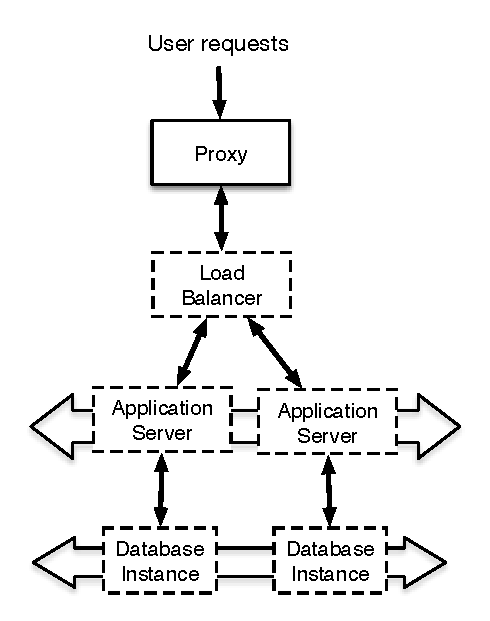
\includegraphics[width=0.35\linewidth]{images/architectureWithout}
}
\subfloat[b][with Shuttle]{
    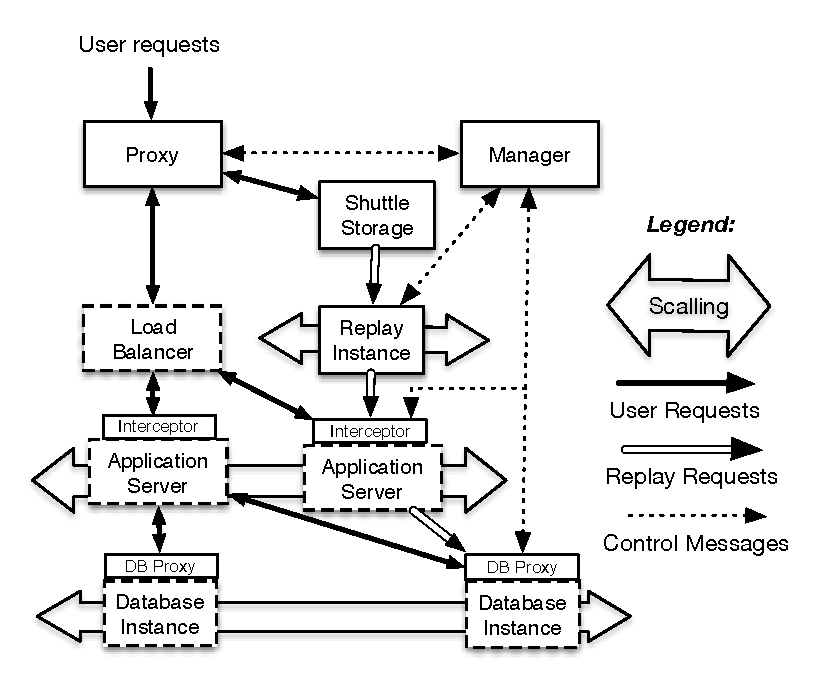
\includegraphics[width=0.55\linewidth]{images/architectureTiers}
}

\caption{Shuttle service architecture:The dashed line components are part of the \ac{PaaS} architecture. The proxy logs the user requests into the Shuttle storage. The manager coordinates the recovery process where the replay instances replay the user requests.}
\label{fig:shuttle_architecture}
\end{figure}
  

%Shuttle Storage
The \emph{Shuttle storage} keeps the content of the user requests and responses. Although we do not consider this aspect in the architecture, this store can be replicated to a remote site to allow tolerating catastrophic failures in a datacenter.


%trusted computing base
We consider the Shuttle components to be part of the trusted computing base since their integrity and availability are critical to recover the application state. We assume that intrusions tamper the application data, which is stored in the database, not the snapshots neither the stored requests. 

%Database
Unlike previous works, our design encompasses distributed databases (\acs{NoSQL}). These databases are designed to scale horizontally. Therefore, Shuttle can also be scaled by adding more database instances.

%How the architecture fits the PaaS
PaaS offerings are supported by a computing infrastructure, often provided as a service (IaaS model), able to scale the application allocating new instances on-demand or automatically, to maintain the quality of service despite demand oscillations. This elasticity  allows allocating replay instances and to scale the application to attend the requests issued by them during the recovery process. Due to the common pay-per-usage model, these resources are paid only when a recovery process occurs. The remaining cost of the service comes from storing client requests and database snapshots. Our design aims to optimize the available resources to reduce the recovery period and costs. 


%%%%%%%%%%%%%%%%%%%%%%%%%%%%%%%%%%%%%%%%%%%%%%%%%%%%%%%%%%%%%%%%%%%%%%%%%%%%%%%%%%%%%%%%%%%%%%%%%%%%%%%%%%%%%%%%%%%%%%%%%%%%
\section{Normal Execution}
\label{sec:arch:normal_execution}
Shuttle logs the data it needs to recover applications during the normal execution phase: user \ac{HTTP} requests, application \ac{HTTP} responses, database items accessed by each request and sequence of operations to each database item (Figure \ref{fig:normal_execution}). In this section, we describe the normal execution phase following the path that a request takes to be processed.

\begin{figure}
\centering
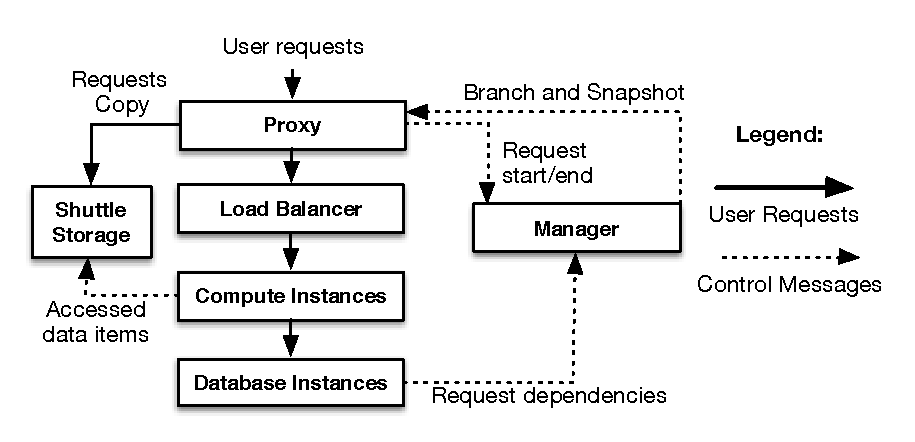
\includegraphics[width=130mm]{images/normalExecution}
\caption{Interaction between components during the normal execution}
\label{fig:normal_execution}
\end{figure}

%Proxy
The proxy intercepts all user \ac{HTTP} requests, except those to static contents (e.g., images), and adds a new header field named \ac{SRD}. Each \ac{SRD} contains three subfields: \ac{RID}, which is an unique timestamp; \emph{Branch} and \emph{Snapshot}, which define, respectively, the database branch and snapshot (Section \ref{sec:arch:snapshot}) and a \emph{restraint} flag, which is used to support runtime recovery (Section \ref{sec:arch:runtime_recovery}). 

The proxy also intercepts every application response, associates the response with the original request and adds a new timestamp to track the ending of the request execution. Requests, responses and their timestamps are stored in the \emph{Shuttle storage} using asynchronous I/O, which permits the operations to proceed before the transmission has finished. 

Requests are sent to the load balancer, which forwards the requests through the application instances according to their usage.


%Application instance
The application instances invoke the database service using the database client library. The database client library intercepts the operations, logs the accessed data items per request and stores this information in the \emph{Shuttle storage}. The database invocation is tracked at client side because the database may not be available or operations may fail.

%Database
On each database instance, the database proxy logs the operations' \ac{RID} and type. The sequence of operations to a data item defines its \emph{operation list}. Periodically, each database instance iterates the operation list of every data item to establish the dependencies between requests. Shuttle also performs snapshots periodically. The snapshot operation stores a new version of data item on the next write operation (Section \ref{sec:arch:snapshot}).


%Summary
In summary, every request-response pair is timestamped and logged by the proxy, the application instances the accessed data items per request, the database logs the sequence of operations per data item. The sequence of operations of each data item is kept in the database instance in which the data item is stored. The remaining data is stored in the \emph{Shuttle storage}, which can be located, or replicated, in a remote site to prevent catastrophic disasters rebuilding the application state using the requests and a previous snapshot. The manager retrieves, asynchronously, the requests' start and end timestamps, which are sent by the proxy, and their dependencies, which are collected by the database instances. Shuttle uses the information retrieved to generate the request dependency graph (Section \ref{sec:arch:dependencies}). 






%%%%%%%%%%%%%%%%%%%%%%%%%%%%%%%%%%%%%%%%%%%%%%%%%%%%%%%%%%%%%%%%%%%%%%%%%%%%%%%%%%%%%%%%%%%%%%%%%%%%%%%%%%%%%%%%%%%%%%%%%%%%
\section{Recovery}
\label{sec:arch:recovery}
%how we will recover?
The intrusion recovery process consists of three steps. The first step concerns the intrusion detection, in which tenants detect intrusions, suspicious behaviors or software flaws. Tenants may use automated tools such as \ac{IDS} \cite{itdb} to detect intrusions. The second step is vulnerability management in which vulnerabilities are identified, classified and mitigated. This work assumes that tenants identify the malicious requests (the subsequence of actions $A_{intrusion}$ whereby the attacker compromises the application) correctly and modify or remove them. Alternatively, tenants can provide an updated and vulnerability-free software version (Section \ref{sec:arch:detection}).
In addition, Shuttle provides several methods to help tenants to identify the malicious requests: determine the set of requests that accessed a set of affected database entries  after an estimated intrusion moment; group requests by user-session; compare database versions to check if the vulnerabilities are correctly mitigated.

The third step consists in removing the intrusion effects. Intrusions affect the application integrity, confidentiality and/or availability (Section \ref{sec:related:recovery}). Recovery from confidentiality violations is out of the scope of this document. However, we argue that the design of the applications should encompass cryptography techniques which may reduce data relevance and protect the data secrecy \cite{Maheshwari2000}.
Shuttle aims to recover applications from integrity violations, which often harm the availability. Shuttle can accomplish some of the goals of intrusion tolerance, keeping the application availability. Applications can keep providing a, possibly degraded but adequate, service during the intrusion recovery. Incoming requests are executed while the recovery process occurs without externalization to users (Section \ref{sec:arch:runtime_recovery}). In addition, Shuttle reduces the system downtime by reducing the time to recover when intrusions happen. Shuttle does not replace the intrusion prevention, detection and tolerance mechanisms, which are the primary lines of defense against attacks.\\

In order to remove the intrusion effects, Shuttle loads a database snapshot, which is selected by the tenant. The selected snapshot shall be previous to the intrusion moment in order to replace the value of every data item by a non-tampered value. Shuttle \textit{manager} orders the \ac{PaaS} controller to launch a new set of application instances and deploys an updated source code version, which may include code fixes. Then, the manager orders the database instances to load the selected snapshot (Section \ref{sec:arch:image_rejuvenation}). The application is intrusion-less now that the snapshot is previous to the intrusion and the application is redeployed on new instances. 

After, the manager initiates a set of \textit{replay instances} to replay the legitimate requests of the sequence of legitimate actions that happen after the snapshot, $A-A_{snapshot}-A_{intrusion}$. The replay instances retrieve a list of requests to replay and get the requests \ac{HTTP} package from the \emph{Shuttle Storage} (Figure \ref{fig:replay_execution}). Most \ac{PaaS} systems scale automatically and horizontally, i.e., they increment or decrement the number of containers based on the measurements of the containers usage. Therefore, the application-logic and data tiers scale to attend the requests from the replay instances, increasing the recovery speed.

The database separates the versions used by the replayed requests and the new requests, preventing the application from exposing a downtime. After the recovery process, the new requests are also forwarded to the recovered database version (Section \ref{sec:arch:runtime_recovery}).\\


The main version of Shuttle loads a previous database snapshot and replays every legitimate user request. An algorithm concerning selective replay is introduced in Section \ref{sec:arch:selective_replay}. \\

In the following sections, we discuss each of key process of the recovery phase in further detail.

\begin{figure}
\centering
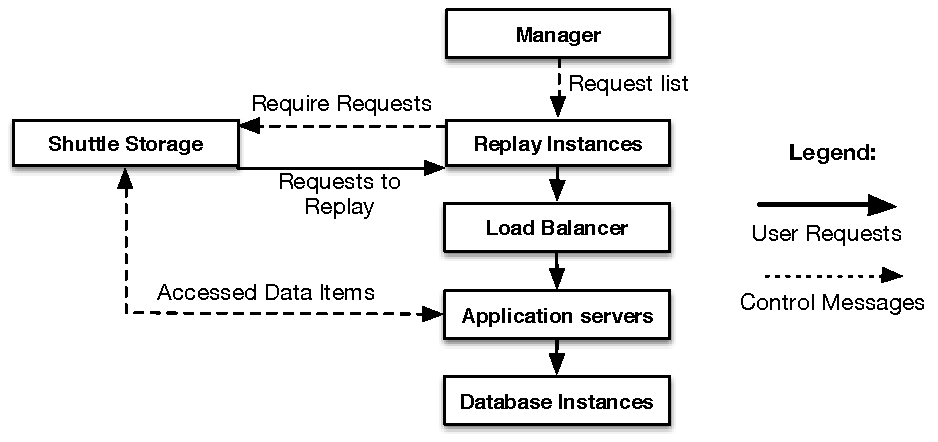
\includegraphics[width=110mm]{images/replayExecution}
\caption{Interaction between components during the recovery process}
\label{fig:replay_execution}
\end{figure}









%%%%%%%%%%%%%%%%%%%%%%%%%%%%%%%%%%%%%%%%%%%%%%%%%%%%%%%%%%%%%%%%%%%%%%%%%%%%%%%%%%%%%%%%%%%%%%%%%%%%%%%%%%%%%%%%%%%%%%%%%%%
\subsection{Intrusion and vulnerability correction}
\label{sec:arch:detection}
%how the damage is fixed?
The recovery process starts when intrusions are detected or the application software requires an update. Intrusion detection is out of the scope of this work. We assume that tenants, or system operators, detect one or more intrusions with the following sources:

\begin{enumerate}
\item User request (e.g. stolen user session)
\item External action: actions not logged by the proxy (e.g. ssh connection to the instances)
\end{enumerate}

Attacks may:
\begin{enumerate}
\item Tamper the database (e.g. adding new entries)
\item Tamper the container (e.g. changing the deployed application in the container)
\end{enumerate}

Shuttle supports the following actions to fix the exploited vulnerabilities:
\begin{enumerate}
\item Update the application software
\item Identify a set of tampered database entries
\item Add, modify or remove logged requests
\item Launch cleaned database or application server instances
\end{enumerate} 

Shuttle removes these effects of malicious actions redeploying the application in new containers and rolling back the database to a snapshot previous to the intrusion.

Attackers may use external actions to perform the intrusion, for instance gaining control of the instance to modify the database files. These actions are not recorded by Shuttle therefore they are not replayed and the application recovers a consistent state. We analyze several intrusion scenarios in Section \ref{sec:eval:accuracy}.\\


If tenants update the application software, they have to ensure that the application's interface remains compatible with the requests that will be replayed. Alternatively, tenants may update the entries in the database and provide a script to modify the requests make them compatible with the new \ac{API}. 

If the database is tampered using user requests, the tenant has to identify the malicious user requests. In addition,tenants can provide the set of suspicious database entries to Shuttle and it will resolve the set of requests that accessed the suspicious items after the estimated intrusion moment. Knowing the suspicious requests, the tenants shall use Shuttle to add, modify or remove the past requests to remove accidental or malicious behaves. \\

In summary, at the beginning of the intrusion recovery process, tenants shall ensure that:
\begin{enumerate}
    \item The software is correct: previous flaws are fixed, its \ac{API} is compatible with the requests and its behavior is the expected.
    \item The requests, which are selected to replay, are legitimate and their dependencies are correct.
    \item The estimated intrusion moment is previous to the intrusion moment (the selected snapshot is intrusion free).
\end{enumerate} 


%%%%%%%%%%%%%%%%%%%%%%%%%%%%%%%%%%%%%%%%%%%%%%%%%%%%%%%%%%%%%%%%%%%%%%%%%%%%%%%%%%%%%%%%%%%%%%%%%%%%%%%%%%%%%%%%%%%%%%%%%%%%
\subsection{Snapshot}
\label{sec:arch:snapshot}

%Why I need a snapshot? To reduce the work during replay.
Shuttle needs to remove intrusion effects. In Section \ref{sec:related:recovery}, we presented two mechanisms to do so: record the data item values or compensate the malicious actions. The first makes a copy of the data item value at a certain instant $t$, implying more storage resources. The second applies compensating actions to each action over the data item value after the instant $t$, which requires more computation resources to invert every action after $t$. However, the compensation mechanism requires the knowledge of the actions that revert the effects of the malicious actions. Moreover, if a malicious action is not recorded, then compensation mechanisms do not revert its effects. Since the set of operations is unknown and Shuttle aims to remove all intrusion effects, we perform snapshots by recording the value of the database items at a certain instant $t$ (first mechanism).\\

%What is a snapshot
A snapshot is a complete set of versions of every data item in the system from which data values can be read but to which updates are not made. Snapshots save the application persistent state at a certain moment. Unlike the selective undo approach, which only reverts the tainted data items (Section \ref{sec:arch:selective_replay}), the full replay approach loads a snapshot previous to the intrusion instant. This approach reverts every database item and removes the effects of any action that occurred after the snapshot creation. \\

%How it is useful?
The duration of the recovery process is mainly defined by the number of requests previous to the intrusion of the set, $A_{before}$. The snapshot mechanism avoids to replay every request from the beginning of the application, which can take too long. Shuttle requires not only a snapshot but also every action posterior to the snapshot instant. Therefore, Shuttle keeps every user request posterior to the oldest stored snapshot instant. The snapshot period defines the usage of storage and computation resources. We argue that tenants can balance the costs of storage and computation resources by specifying a policy to perform the snapshot. The policy shall consider the rate of requests, the data written per request, the expected time to detect the failure and the application capability to provide an possible degraded service during the recovery period. \\

%What Shuttle needs to do?
Shuttle takes snapshots automatically and according to specified policies. It records the persistent state of the application, i.e., the database values, at a certain instant. The volatile state of the application, for instance its stack, is not stored as we consider the web servers to be stateless. \\


%Request consistent snapshots
Performing snapshots in distributed databases is not trivial since snapshots have to be consistent with the user requests.  We consider each user request may include multiple database operations, each of them to multiple database servers, without using transactions. Consequently, the sets of database operations of each user request cannot be aborted and do not have a global order. If Shuttle replays requests on a snapshot that contains part of the persistent state written by a request during its first execution, the replay will be inconsistent. The database must reflect the effects of a set of completed requests and not the results of partially executed requests. Therefore each snapshot shall be \emph{global request consistent} containing either all or none of the database updates made by every request.


We define \textit{request consistent global snapshot}: a snapshot is global request consistent if it records a state of the database which reflects the effect of a set of completed requests and not the results of any partially executed request. This concept derives from the notion of \emph{transaction consistent global checkpoint}: a checkpoint is a transaction-consistent global checkpoint if it contains all or none of the updates made by a transaction \cite{global-checkpoint}. Since most \acs{NoSQL} databases do not support transactions, we extend the concept of transaction to \textit{request transaction}. A request-transaction embraces all database operations performed due to the execution of a request. Unlike \ac{ACID} transactions, a request-transaction may not be possible to abort. In summary, Shuttle snapshots are request consistent: a snapshot contain all or none operations of a request.


%Log-oriented vs dump-oriented vs Fuzzy
Checkpointing algorithms for distributed databases can be classified as log-oriented and dump-oriented \cite{checkpoint-survey}. In the dump-oriented approach, the checkpoint is referred to as the process of saving the state of all data items in the database. In the log-oriented approach, periodically a dump of the database is taken and also a marker is saved at appropriate places in the log. When a failure occurs, the latest dump is restored and the operations on the log after the dump was taken is applied to the dump until the marker is reached to restore the database to a consistent state \cite{global-checkpoint}. We take the latest approach.\\


In addition, the snapshot mechanism shall be non-blocking: the processes shall not stop their execution while taking snapshots.  

%Straightforward solution
A straightforward way to take a request-consistent global snapshot is to stop processing new requests, waiting until the currently executing requests finish, then making a copy of each data item. However, this solution incurs on communication overhead to reach a globally inactive state and causes application downtime. Yet, this approach may fit applications that can be unavailable during a certain period, for instance, during a certain period of the night. \\


Kim and Park \cite{kim_checkpoint} propose an approach in which a coordinator broadcasts a checkpoint-request message to every database node. Each database node divides the transactions into two groups: before the checkpoint-request $T_p$ and after $T_f$. Updates of transactions in $T_p$ are flushed to the current database, while the ones in $T_f$ are flushed in a \emph{checkpoint area} (a temporary allocated storage area). When all transactions of $T_p$ are done, the checkpoint area is updated with items updated by transactions in $T_p$ but not by $T_f$. After, the rules of current database and checkpoint area are exchanged. The major drawback of this approach comes from updating the checkpoint area: the database is unavailable during the updating process.


%Our solution
Our solution leverages the existence of a single load balancer and, consequently, single proxy that adds a \ac{SRD} field to every request. Every \ac{SRD} contains a \ac{RID}, an unique and incremental identification of each request given by the instant when the request is retrieved. Every database operation is identified by the \ac{RID} of the source user request.

In order to create a snapshot, tenants define a future instant in time $t$ when the snapshot will occur. The instant, named \ac{SID}, identifies the request-consistent global snapshot. The manager passes the \ac{SID} to every database proxy.

Database proxies use the \ac{SID} to define the version of the data item used by the operations. Operations with \ac{RID} lower than the scheduled snapshot instant (\ac{RID} < \ac{SID}) access the version before the snapshot. Otherwise, the operations access the latest data item version. This mechanism splits requests to accomplish a request-consistent global snapshot, and allows tenants to schedule snapshots without application downtime. Figure \ref{fig:snapshots} illustrates the sequence of 7 database operations on the database item $x$ and 3 snapshots (excluding the base snapshot).

\begin{figure}
\centering
  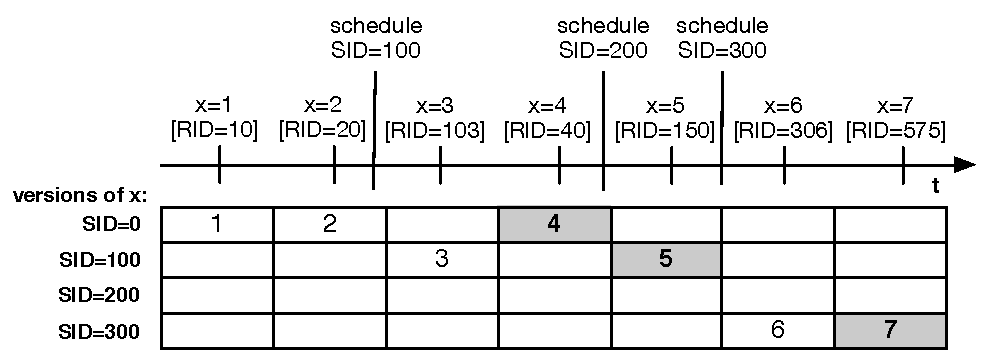
\includegraphics[width=130mm]{images/snapshots}
  \caption[Snapshot versions stored in the database]{Versions stored in the database during a sequence of 7 operations and 3 snapshots. The final values of the stored versions are contained in filled squares. The tenant schedules 3 snapshots on SID: 100, 200, 300.}
\label{fig:snapshots}
\end{figure}

In order to avoid to replay every database operation to obtain the snapshot, the snapshot mechanism shall create a database copy (dump). We avoid blocking the application to copy values using a copy-on-write and incremental method. When a data item is written for the first time in each snapshot, Shuttle creates a new version of the data item. Since a data item may not be written in every snapshot, e.g., $SID=200$ in Figure \ref{fig:snapshots}, we associate a \emph{version list} to every data item. A \emph{version list} tracks on which snapshots the data item has been written. In conclusion, the snapshot is an incremental mechanism because it does not require to duplicate data.\\
%The version list also contains read requests that did not succeeded, for instance when the data item does not exists, to avoid false positives. 


%Particular case
A snapshot might become inconsistent. For instance, Table \ref{tab:snapshot_caso_bicudo} represents the execution of two concurrent requests. Their normal execution is consistent. A snapshot with \ac{SID}=5 would contain [A1 = 11] and be a global request-consistent. However, if Shuttle loads the snapshot and replays the request 20, its first read operation reads A1 == 11 instead of A1 == 10. 


This particular case happens when a request with \ac{RID} greater than the snapshot instant \ac{SID} read a version belonging to the snapshot \ac{SID} and, after, a request with \ac{RID} lower than \ac{SID} overwritten that version. Storing a new version and adding a flag on the version list solves the problem. Nevertheless, we expect this to happen only in rare occasions.

%the  and every operation with \ac{RID} > \ac{SID} reads/writes the new version. Operations of requests with \ac{RID} > \ac{SID} that read the original value, for instance A = 10, are marked and read the old version during the replay. 
%in parallel during the transition period, i.e., when a request accesses the previous snapshot and other accesses the current snapshot. 


\begin{table}
\centering
\begin{tabular}{l|l|l}
\textbf{RID=10 (SID = 1)}     & \textbf{RID=20 (SID=15)}   & \textbf{Storage}\\ \hline
Write A=10                    & ~                          & A1=10  \\
~                             & Read A: A1==10             & A1=10  \\         
~                             & Write A=20                 & A1=10, A15=20 \\
Read A: A1==10                & ~                          & A1=10, A15=20 \\
~                             & Read A: A15==20            & A1=10, A15=20 \\
Write A=11                    & \textit{Completed}         & A1=11, A15=20 \\
\textit{Completed}            & ~                          & A1=11, A15=20 \\
\end{tabular}
\caption[Concurrent requests]{Concurrent requests: the snapshot instant is 15, the left request accesses data previous to the snapshot (A1) while the right accesses the latest (A15 or A1). }
\label{tab:snapshot_caso_bicudo}
\end{table}


%Discussion
Unlike the approach proposed by Kim and Park, our approach allows to record multiple snapshots keeping various data item versions and does not require to copy the transactions.

The value of \ac{SID} must be known by every database instance before the execution of any request with $RID > SID$. If the \ac{RID} was determined by incremental request counter, then Shuttle would need to analyze the request rate and estimate the \ac{SID} value. However, the request rate can vary and the snapshot would fail. Notice that our mechanism does not require clock synchronization because the \ac{RID} is defined by the proxy timestamp and tenants can schedule a snapshot defining a future time instant. The period between the scheduled moment and the present must be bigger than the communication delay between the manager and the database instances. Consequently, we assume the communication between the manager and database proxies is synchronous: the messages are delivered within a fixed time.


%%%%%%%%%%%%%%%%%%%%%%%%%%%%%%%%%%%%%%%%%%%%%%%%%%%%%%%%%%%%%%%%%%%%%%%%%%%%%%%%%%%%%%%%%%%%%%%%%%%%%%%%%%%%%%%%%%%%%%%%%%%%
\subsection{Dependency Graph}
\label{sec:arch:dependencies}
%Dependency definitions
An application execution can be modeled as a set of actions and a set of objects. Actions read and write objects. An action $A$ is dependent from an action $B$ if $A$ reads an object's version written by $B$.

%why is relevant in general
Requests must be replayed in a consistent manner to obtain a consistent application after the replay phase. The request replay order must ensure that if the requests, application semantics and initial database values are the same, then the final database values are equal. For this propose, the dependencies between actions shall remain consistent: if during the first execution an action $A$ becomes depends on an action $B$ by an object $O$, then during the replay phase $A$ shall read the object $O$ only after $B$ updates the object $O$. Otherwise, $A$ may read a version different than the original version.

%related work and why it does not work in PaaS
Previous proposals, for instance \emph{in} \cite{goel}, leverage the request serialization provided by snapshot isolation in relational \ac{DBMS} to order the operations to replay. In contrast, \textit{Undo for Operators} \cite{undoForOperators} uses the application protocol knowledge to establish the dependency between requests and order them. However, accesses to \acs{NoSQL} databases are not globally serialized. Moreover, the data items accessed during the replay phase may change due to updates to the application semantics, request modification or multi-threaded execution. At last, the application semantics is unknown in advance since we want to support any application deployed on \ac{PaaS}. Taking that into account, we propose a novel approach.\\


%Rules
Shuttle tracks the dependencies between actions in a \textit{dependency graph}. A \emph{dependency graph} consists of nodes that represent requests and edges that establish dependencies between them (Figure \ref{fig:selectiveGraph}).  Dependencies between requests are established using the following rules: a request $R_A$ is dependent upon request $R_B$ if there is a data item $x$ such that $R_A$ reads $x$ and $R_B$ performs the latest update on $x$ before the read operation by $R_A$. Dependencies are transitive except when requests perform blind writes, i.e., requests write items without reading them first \cite{Ammann2002}. Therefore, the dependency graph is a mixed graph, if there is a dependency between $A$ to $B$, then there may be a dependency between $B$ and $A$.


%How Shuttle creates the dependency graph?
Previous solutions for relational databases extract the dependencies using a pre-defined, manually-created, per-transaction type template \cite{itdb}, or change the relational database management system code to extract read dependencies \cite{phoenix}. In contrast, Shuttle uses the database proxy to log the database accesses. Periodically, each database proxy traverses, in background, the \emph{operation list} of each data item to collect the new accesses and to generate the dependencies between requests. The Shuttle manager processes the dependencies to update the dependency graph. An alternative approach is to pull the dependencies from each database node only before the recovery process and generate the dependency graph when needed. 






%false positives: detected but not exist
The above method may lead to \emph{false positives}, i.e., to flag dependencies that do not exist. For instance, a request may read a data item but not use it to compute the written value, so there is no real dependency. Although tracking variables used by each request during its execution might solve this particular case \cite{goel}, it would require modifying the code interpreter (e.g., Zend Engine for PHP), which would constrain Shuttle to a set of specific languages. As our approach uses the dependencies to group the requests that can be executed concurrently, false dependencies imply a performance penalty but do not cause data loss or inconsistent state. On selective replay mode, the dependency graph is used to determine the tainted requests and the request that need to be replayed. Again, false dependencies only harm the performance.

When tenants use the dependency graph to determine the set of malicious requests, $A_{malicious}$, they shall take into account that false dependencies may lead to consider legitimate operations as malicious and, consequently, cause data loss.

%false negatives: not detected but exist
Complex queries on a relational database may lead to \emph{false negatives}, i.e. a dependency exists but is not detected. For instance when a read operation would have been executed on a deleted data item if this data item had not been deleted before the request execution \cite{Xie2008}. Therefore, legitimate transactions may have different output even when they were not affected by malicious execution during their original execution. Since user mistakes are often delete operations due to wrong query arguments, this is a relevant issue. 

In contrast with SQL queries that access the data items that match a query, the \ac{CRUD} interface of most key-value stores specifies, in a deterministic and apriori manner, the data item that will be accessed. Shuttle logs every access, even when the data items do not exist, keeping the \emph{operation list} of the deleted data items to track further operations.\\


%Cycles
%Each request may perform multiple database operations, each of them to multiple database servers, without defining a global \ac{ACID} transaction. 
Shuttle can not replay requests synchronously, i.e., waiting for the response to the previous request before sending the next. To replay the requests synchronously would not have only performance degradation but also lock the replay phase because requests, which have been originally executed in concurrently during the normal phase, may be depend on each other. Therefore, Shuttle replays requests asynchronously and, hence, concurrently. Two requests are executed concurrently if they are dependent from each other. For instance, Figure \ref{fig:inconsistency_db_order} represents the first execution of two requests that increment the variable $A$. The $Request 1$ depends on $Request 2$ and vice versa. 

%Ordering using operation list
Yet, re-execution of concurrent requests is not deterministic. User requests are processed concurrently using multi-threaded servers and the system messages, including database requests, do not have a delivering order. Therefore, the execution order of two concurrent requests is unknown. To deal with this issue, our novel approach uses the \emph{operation list} to turn the re-execution of concurrent requests deterministic. An \emph{operation list} is a sorted list that records the operations to a data item. During the replay phase, the operations to a data item must follow the order established by is operation list. For instance, in Figure \ref{fig:inconsistency_db_order}, the operation list of the data item $A$ is: $[Req1:Get, Req1:Put, Req2:Get, Req2:Put, Req1:Get, Req1:Put, Req2:Get, Req2:Put]$. {Req.~1} and {req.~2} are replayed concurrently but the result is consistent because the order is established by the operation list.

%Unlocking
During the recovery period, intrusions are removed and the application code is updated. This may cause requests to access different data items than in the first execution. Requests may not access the same sequence of data items or read/write the same content. If an operation contained in the operation list is not performed, the following operations to the data item are blocked and the request fails. To address this problem, at the end of each request execution, the \textit{database client interceptor} fetches the list of data items accessed by the request on its first execution and compares them against the ones accessed during the replay process. The database client library invokes the \emph{database proxy} with the data items that have not been accessed to unlock the operations of the remaining requests. 

For instance in Figure \ref{fig:inconsistency_unlock}, the $Request 1$ has a different replay execution performing $B = B \times 5$ instead of incrementing $A$. The second operation of {req.~2} is delayed until the end of the {req.~1} because it succeed the second operation of {req.~1} in the operation list. After the execution of {req.~1}, the database client interceptor unlocks the second operation of {req.~2}.\\

\begin{figure}[!htb]
\hspace*{-3mm}
\mbox{
  \subfloat[][Ordered by the operation list \label{fig:inconsistency_db_order}]{
      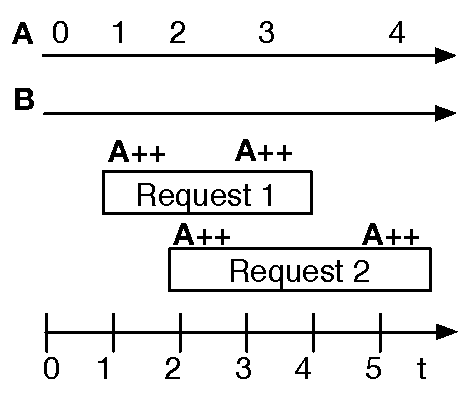
\includegraphics[width=0.25\linewidth]{images/inconsistency_db_order}
  }

  \subfloat[][Operation unlock \label{fig:inconsistency_unlock}]{
      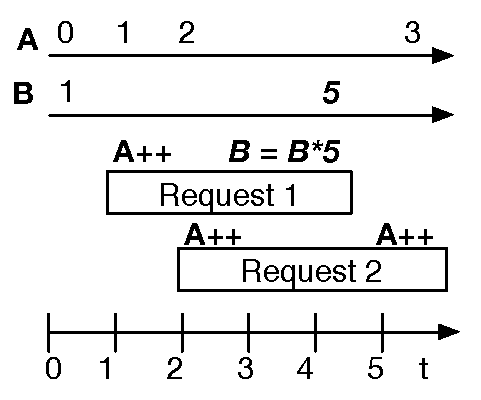
\includegraphics[width=0.25\linewidth]{images/inconsistency_unlock}
  }

  \subfloat[][Consecutive requests \label{fig:inconsistency_serial}]{
      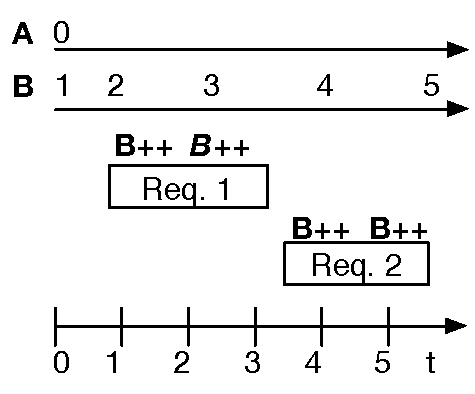
\includegraphics[width=0.25\linewidth]{images/inconsistency_serial}
  }

  \subfloat[][Conflict \label{fig:inconsistency_conflict}]{
      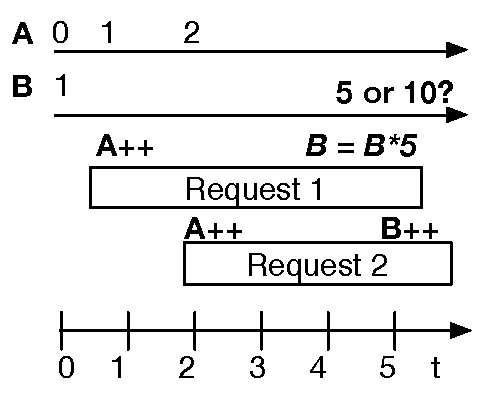
\includegraphics[width=0.25\linewidth]{images/inconsistency_conflict}
  }
}
\caption{Replay two requests with different re-execution}
\label{}
\end{figure}


%New dependencies during the recovery time
During replay there may be non-deterministic situations, whenever an access is not contained in the operation list. The most complex scenario during the replay is when two requests, originally executed in parallel, access different data items comparing with their first execution, establishing a new dependency. The result is unpredictable. Consider the possible re-execution in the Figure \ref{fig:inconsistency_conflict} where the {req.~2} increments $B$ simultaneously with {req.~1} performing $B = B \times 5$. The result is unpredictable because the {req.~1} may write before or after {req.~2}. Since both requests did not access the data item $B$ during their first execution, the operation list does not establish an access order. Therefore, the {req.~1} and {req.~2} may execute on a arbitrary order. The order of these requests is as deterministic as if during the first execution: the operation of \emph{req.~1} can execute before, between or after \emph{req.~2}.


%naive
A naive solution would be to detect the new dependency during the replay process, stop the process and start a new replay process in a new snapshot, including the new dependency.

%brown
Brown \textit{et al.} \cite{undoForOperators} propose the concept of \textit{verb} (Section \ref{sec:related:recovery_app}). A verb object encapsulates a single interaction (request/response) of the user and exposes an interface to establish the order between requests and their dependencies. However, tenants shall know the applications' operations to create the verbs defining: a commutativity test, an independence test, a preferred-ordering-test and an application-defined action to handle a inconsistency if the operation fails. Since Shuttle shall support any \ac{PaaS} application, the applications' semantics are unknown in advance. Therefore, this solution is not adequate.

%sorted log
A sorted-log, in which the accesses are sorted, for instance by \ac{RID}, would establish that operations must have a strict incremental order. However, operations with smaller \ac{RID} than the previous are aborted. For instance, the second operation of {req.~2} in Figure \ref{fig:inconsistency_db_order} would be aborted.

%sorting per start-end
An alternative solution consists on sorting the requests per \emph{start-end order}, instead of using the dependency graph. A request starts only after all requests with end lower than it ends. Dependencies between requests remain correct, since they are constrained by the \emph{operation list}. Thus the parallel requests are ordered and replayed in a similar manner to the first execution. Two serial requests can have distinct re-executions: if a request starts after the end of the previous. For instance in Figure \ref{fig:inconsistency_serial}, {req.~1} and {req.~2} can have distinct re-executions.

If two operations are re-executed concurrently, then their order is as deterministic as if they happen during the first execution. For instance in Figure \ref{fig:inconsistency_conflict}, the operation of {req.~1} $B = B \times 5$ is executed in parallel with the operations $B++$ of {req.~2}. The order of these requests is as deterministic as if during the first execution: the operation of {req.~1} can execute before, between or after {req.~2}.


%version and semantic reconciling
In order to turn more operations of the replay process consistent with the first execution, we can leverage semantic reconciliation, as \textit{in} Dynamo \cite{Decandia2007}. The case represented in Figure \ref{fig:inconsistency_conflict} is equivalent to a concurrent update where two parallel writes are performed on distinct database instances. Each request writes a distinct version resulting in conflicting versions of an item. Developers use the application-assisted conflict resolution interface to merge the versions (reconciliation) \cite{Decandia2007}. In this case, the following read operation would access the values written by the latest operation. For instance, if the latest is {req.~1}, then it choose between $1$ and $2$. If the latest is {req.~2}, then it choose between $1$ and $5$. This solution can produce a consistent output.\\

In summary, unlike previous solutions, Shuttle orders the requests using their start and end instants and constraining the operations to the order established on the \textit{operation lists}. This approach allows requests to access new data items during the recovery process and to replay concurrent requests.





%%%%%%%%%%%%%%%%%%%%%%%%%%%%%%%%%%%%%%%%%%%%%%%%%%%%%%%%%%%%%%%%%%%%%%%%%%%%%%%%%%%%%%%%%%%%%%%%%%%%%%%%%%%%%%%%%%%%%%%%%%%%
\subsection{Clustering}
\label{sec:arch:clustering}

Despite Shuttle's capability to replay concurrent requests, one of the main challenges of Shuttle is to reduce the recovery period. We assume that critical software flaws and intrusions can be detected in a short period of time, from seconds to one week. If a fault exists during a longer period, then the application may tolerate a longer recovery phase because the recovery process used by Shuttle does not require application downtime (Section \ref{sec:arch:runtime_recovery}). Still, we want recovery to take a fraction of the time elapsed since the snapshot from which recovery starts (e.g., if the snapshot was taken a week before, we want recovery to take much less than that period).  

We address this problem grouping the requests into \emph{clusters}. A cluster is a set of requests that have dependencies between them but not from/to requests in other clusters. Clusters are created when the recovery is about to start by inspecting the dependency graph. Since clusters are independent, they are executed concurrently by different \emph{replay instance} without synchronization. Requests within the same cluster, are performed in start-end order (Section \ref{sec:arch:dependencies}). Given that more requests are executed concurrently, Shuttle launches more application servers and database instances to process the replayed requests. Therefore, the replay phase throughput is bigger than the during first execution and the recovery time is minimized. This mechanism is applicable if the graph dependencies remain unchanged during the recovery phase, i.e,. every replayed operation is contained in the operation list but not all operations in the list must be replayed.

Taking the above in account, we define two replay approaches: \emph{serial replay} and \emph{parallel replay}. The first considers every request in the same cluster. The later uses the dependency graph to group the requests in independent clusters. Both approaches replay the requests in start-end order, supporting concurrent requests \ref{sec:arch:runtime_recovery}. In contrast to \emph{serial replay}, \emph{parallel replay} allows to perform more requests in parallel but it does not support new dependencies during the replay phase. Therefore, \emph{parallel replay} requires that tenants ensure that the dependencies between requests do not change during the replay process. Since the dependencies between requests often remain constant and novel dependencies are easily detected, we consider \emph{parallel replay} represents a significant advantage for \ac{CSP}. These approaches are compared in Chapter \ref{chapter:evaluation}.




%%%%%%%%%%%%%%%%%%%%%%%%%%%%%%%%%%%%%%%%%%%%%%%%%%%%%%%%%%%%%%%%%%%%%%%%%%%%%%%%%%%%%%%%%%%%%%%%%%%%%%%%%%%%%%%%%%%%%%%%%%
\subsection{Instance Rejuvenation}
\label{sec:arch:image_rejuvenation}

% Why? Instances can be corrupted
\ac{PaaS} systems launch instances/containers and deploy applications or databases on them. Attackers may exploit vulnerabilities in the instances configuration to affect the service integrity, confidentiality or availability. For instance, an attacker may explore the shellshock vulnerability in the GNU's bash shell of out of date instances.

%Related work
An effective technique to remove intrusion effects and restore the application availability is to terminate compromised containers and launch new containers. We name this approach as \textit{instance rejuvenation}. A similar approach is used in proactive recovery systems for Byzantine fault tolerance. Castro \textit{et al.} \cite{Castro2002} propose a mechanism that recovers the replicas of a system periodically even if there is no reason to suspect that they are faulty. This mechanism aims to prevent an attacker from compromising the service by corrupting a quorum of the replicas without being detected. We extend this approach to \ac{PaaS} to remove possible intrusion effects in containers, even if there is no reason to suspect that they are affected by the intrusion.\\



%How it works?
Shuttle interacts with the \ac{PaaS} controller rejuvenate instances when they are compromised and a new recovery process begins. This process launches new instances. The \ac{PaaS} controller initializes the new instances with updated container images and deploys an updated version of the application code or database, which may include updates to fix discovered flaws or prevent future intrusions. Shuttle copies the snapshot selected by the tenant to new database instances. Requests are replayed on the novel instances while the incoming requests are processed by the old instances, perhaps with a degraded integrity constrains. This mechanism keeps the application available during the recovery process. After the recovery process, the old instances are terminated.\\

%Why its good?
We assume new instances to be intrusion-free since tenants or CSPs can update the image and the image is installed on an empty persistent-state. This approach fits the concept of automatic deployment applications in \ac{PaaS}. Applications for \ac{PaaS} platforms are designed to scale horizontally so the number of application instances can be dynamic.

%remote replication
In addition, the instances can be instantiated in a remote site to recover from catastrophic disasters \cite{cloud-disaster}. Snapshots, database operation lists, application code and requests can be replicated to a remote site. If they are available, then Shuttle can launch new instances on a remote datacenter, deploy the application code, load the snapshot and operation lists in the database instances and replay the requests. This is a log-based recovery process \cite{Wang2010} that allows to recover the  application integrity and availability.

%software testing
This process can also be used in a proactive manner to renew instances to remove unknown intrusions \cite{Castro2002,Sousa2010} or to test new application versions with user requests to compare its results against the previous version, using the branching mechanism  (Section \ref{sec:arch:runtime_recovery}).

%Consistency
Tenants are responsible for ensuring that request dependencies are correct and the {API} of the updated code version is compatible, or for providing a script to update each request to the new \ac{API}. Moreover, the selected snapshot must be consistent according to the specification of the updated version or every request executed since the application begin shall be replayed.



%%%%%%%%%%%%%%%%%%%%%%%%%%%%%%%%%%%%%%%%%%%%%%%%%%%%%%%%%%%%%%%%%%%%%%%%%%%%%%%%%%%%%%%%%%%%%%%%%%%%%%%%%%%%%%%%%%%%%%%%%%%%
\subsection{Runtime Recovery}
\label{sec:arch:runtime_recovery}

%Goal
Applications shall remain available during the recovery process, perhaps with a degraded behavior, without exposing downtime to users. To do so, Shuttle considers each recovery process defines a new branch, a model inspired in versioning systems such as git \cite{git}.

%How
A \emph{branch} is a sequence of snapshots. Snapshots are analogous to \textit{commits} in git. Each snapshot represents a set of versions of every data item in the database at a certain instant. Each recovery process creates a new branch forking a previous branch on a snapshot chosen by the tenant, either explicitly or implicitly (by indicating the initial intrusion instant, selecting implicitly the preceding snapshot). When a new branch is created, a new snapshot is also created on the new branch. Incoming user requests access only the data of the previous branch keeping the application available, while replayed requests access the created branch without compromising the availability of the application. If Shuttle launches new database instances, then the new branch is created in the new instances and write operations occur in the new instances. Read operations occur in the previous instances until the first write operation of the accessed data item in the new instances.

\begin{figure}
\centering
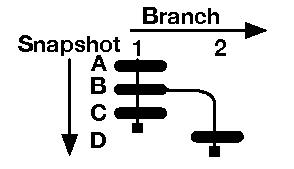
\includegraphics[width=55mm]{images/branches_paper}
\caption[Tree model]{Tree model: 2 branches and 4 snapshots: branch 1 contains the snapshots $A, B, C$; branch 2 contains the snapshot $D$;}
\label{fig:branches_simple}
\end{figure}


%Architecture details
A branch contains a sequence of snapshots but a snapshot can only belong to a single branch (Figure \ref{fig:branches_simple}). Each snapshot represents a possible version of the data item. A novel data item version is created only when the data item is written for the first time during each snapshot. Consequently, the data item may not have a version for each snapshot. Shuttle keeps a list of the versions in which each database item has been written (Section \ref{sec:arch:snapshot}).

%Problem of lack of versions:
For instance, in Figure \ref{fig:branches}, a data item $x$ may have the following sequence of versions on its version list: $[A,B,C,D,E]$. If $x$ has not been written in snapshot $E$, the version $E$ would not exists and the latest version of $x$ would be $D$. However, the snapshot $D$ has been compromised so it is not part of the current branch (branch 3). The latest non-tampered version of $x$ is the version $B$. If version $B$ does not exists, then the latest version is $A$.

%branch path
We define the concept of \emph{branch path}:  a Branch Path of a certain branch is the sequence of snapshots between the current snapshot and the root snapshot. A Branch Path of a certain branch defines the versions available to operations that belong to that branch. The branch path of branch $3$ in Figure \ref{fig:branches} is \{E, B, A\}. The one of branch $2$ is: \{D, C, B, A\}. When a branch is created, its branch path contains the its initial snapshot and the sub-sequence of snapshots in the branch path of the branch of the forked snapshot that are equal or previous to the forked snapshot.

%Version to read
The version accessed by an operation is defined using the branch path of the operation's branch and the version list of the accessed data item: operations read the latest version present in the \emph{version list} and in the \emph{branch path} and write the latest version in the branch path. Therefore, a new version, referring the initial snapshot of the new branch, is added to the version list on the first write operation to each data item during the replay.

%Isolation
This mechanism maps the operations to the correct versions and isolates the multiple, perhaps simultaneous, attempts to recovery the application without compromising the exposed application behavior. During the recovery process, users access the, perhaps corrupted, old branch loaded in the current computation and database instances. Therefore, the application remains online, perhaps with a degraded behavior, without exposing downtime to users.

%Working explanation and switching
At recovery time, the manager sends the new \emph{branch path} to every database instance. The new incoming users access the, perhaps corrupted, old branch while the requests being replace access the new branch. Therefore, the application remains online, perhaps with a degraded behavior, without exposing downtime to users. 

At some point, when the recovery is finishing, the user requests have to start being issued to the new branch. To do so, after replaying the requests, the proxy flag \emph{restraining} is set and every new request is marked with the \emph{restrain} flag. Database accesses marked with \emph{restrain} are delayed. After replaying the requests retrieved during the recovery process, the proxy sets the new branch in the subfield \emph{branch} of \ac{SRD} of the new requests, the \emph{restrain} flag is disabled and the database nodes are notified to proceed the accesses. This mechanism delays the processing of some requests, but this has typically a duration of seconds, compared with a recovery process that may take many minutes or even hours. 

This mechanism ensures the recovery phase to be finite. However, if the rate of requests being replayed is much higher than the rate of new requests, then the requests retrieved during the replay phase are also replayed without restraining new requests. Consequently, the restrain phase is shorter and required only to change branch. 

%Related work, advantages and example
While Aire \cite{retro} used a branching mechanism to perform a recovery process in various systems simultaneously, we propose the mechanism to isolate user accesses from the recovery process. Our model allows the tenants to select any snapshot as base to a new recovery process and create snapshots in different branches. Applications can contain multiple branches simultaneously. Figure \ref{fig:branches} represents an application with 3 branches: the branch 1 is the initial application branch where the tenant made three snapshots ($A$, $B$ and $C$). After detecting an intrusion, the tenant considered that snapshot $C$ is non-tampered and initiated a recovery process based on it creating the branch 2. Afterwards, the tenant made one snapshot ($D$) on branch 2. However, the snapshot $C$ is tampered. So the tenant initialized a novel recovery process based on snapshot $B$ creating the branch 3. In this scenario, the tenant would be unable to recover its application without the branching model. Since tenants may fork a new branch not only from the most recent snapshot. Therefore, the latest non-tampered version of a data item may not be its latest version.

\begin{figure}
\centering
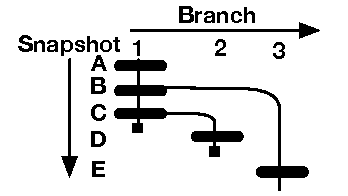
\includegraphics[width=65mm]{images/branches}
\caption[Tree model]{Tree model: 3 branches and 5 snapshots: branch 1 contains the snapshots $A, B, C$; branch 2 contains the snapshot $D$;  branch 3 contains the snapshot $E$.}
\label{fig:branches}
\end{figure}



Inactive snapshots and branches, for instance snapshot $D$ and branch 2 in Figure \ref{fig:branches}, can be deleted to reduce the used storage resources. In addiction, tenants can use the branching mechanism to test their intrusion recovery procedures in background, i.e, without exposing users to test issues.\\

If an intrusion happens during the replay phase, then its effects are stored in the branch of incoming requests. If the intrusion is detected before the restraining flag is set, then the malicious requests are not replayed in the new branch. Otherwise, tenants shall start another recovery process.\\





%%%%%%%%%%%%%%%%%%%%%%%%%%%%%%%%%%%%%%%%%%%%%%%%%%%%%%%%%%%%%%%%%%%%%%%%%%%%%%%%%%%%%%%%%%%%%%%%%%%%%%%%%%%%%%%%%%%%%%%%%%
\subsection{Non-determinism and consistency}
\label{sec:arch:consistency}

Shuttle provides an \ac{API} to handle nondeterminism and inconsistency cases.

%non-determinism: definition
An application is called nondeterministic if two subsequent executions with the same user input cannot be guaranteed to have the same have the same final state and outputs. Five of the main sources of non-determinism in \ac{PaaS} applications are: shared memory, thread concurrency, random number generation, timestamps and message exchanging.

%how non-determinism is handled
We assume requests to be independent thus they do not share memory and concurrent threads are independent. The \ac{API} of Shuttle provides a deterministic random number generation and a timestamp. It uses the \ac{RID}, which is a timestamp set by the proxy, as timestamp and pseudo-random number seed, so the replay of a request will use the same random numbers and timestamp. We consider a single timestamp per request to be enough for most applications. This mechanism is language independent. User requests and database accesses are ordered in a deterministic way using the operation list. Shuttle provides the following \ac{API} for the application developers:

\begin{enumerate}
  \item \textit{getTimestamp():} returns the timestamp (\ac{RID}) set by the proxy (\textit{long}).
  \item \textit{getRandomGenerator():} returns a random number generator that has \ac{RID} as seed.
\end{enumerate}

%User consistency
An important aspect of a recovery system like Shuttle is the application consistency seen by users. For instance, if an user does an action based on data written by a malicious action, which result of the user action replay is consistent. Since users have a non-deterministic behavior, they may have to be notified if a recovery took place and their data was modified. \\


%Related work
%In Undo for Operators \cite{undoForOperators}, operators must specify a compensation action for each request type. 
Since Shuttle is not tied to the application semantics, the actions to compensate the recovery process changes are unknown before the application is created. In addition, the application may contain client-side code, e.g., Javascript, that processes the application responses. For instance, a recover process reorders a list of items. The client-side code may sort the items so the list is seen ordered by users. A replay process taking into account the client-side consistency is proposed in \cite{warp}.


% Compensation API
Shuttle does not execute requests that returned an error in the first execution. We assume that requests are synchronous so users are immediately notified of the error and do not expect that the request will succeed in future. Similarly to other works in the area \cite{undoForOperators}, we assume that these cases are compensated by the user when they happen. As only requests that did not return an error are replayed, Shuttle considers an inconsistency when a request returns an error or a response is different during replay. Shuttle provides the following \ac{API} for the application programmer to define how inconsistencies are dealt with (Shuttle calls these functions in case they are launched by the tenant):

\begin{enumerate}
  \item \textit{preRecover():} invoked before the beginning of the recovery process.
  \item \textit{handleInconstency(request, previous response, new response, previous data items, new data items, action):} invoked when there is an inconsistency.
  \item \textit{postRecover(statistics, old version, new version):} invoked after the end of the recovery process.
\end{enumerate}

The first function allows tenants to perform a set of actions before the beginning of the recovery process, such as notifying the operations team or taking a new snapshot. 
The second function takes as input the operation that caused the inconsistency as well as the response and keys accessed during the normal execution and during the recovery process. It also takes as argument the action to take. Currently we consider three possible actions: 1) ignore the inconsistency; 2) notify the user of the inconsistency; 3) execute another request. This function is invoked, for instance, if a response during the replay is different than the response on the first request execution.
Using the \textit{postRecover} function, the tenant has access not only to the statistics of the recovery process but also to an interface to compare the database values before and after the recovery process and the application responses, before exposing the data to the users. 
Tenants can use this interface to notify their customer to verify their data.
%If tenants aim to determine if a request returned an error in the first execution due to an intrusion, Shuttle can replay the failed requests too.

%External consistency
Besides its users, an application may also interact with external services. We simplify the problem by considering that applications only obtain inputs from external services, disregarding the issue of outputs. The problem is treated in \cite{undoForOperators,aire}. Brown \textit{et al.} \cite{Brown_spheres} models each external service as a recoverable application. During the recovery phase, an external service can also be recovered if its input is distinct. Aire \cite{aire} proposes to initiate a recovery process in the external service and handles the inconsistencies of this process.


%%%%%%%%%%%%%%%%%%%%%%%%%%%%%%%%%%%%%%%%%%%%%%%%%%%%%%%%%%%%%%%%%%%%%%%%%%%%%%%%%%%%%%%%%%%%%%%%%%%%%%%%%%%%%%%%%%%%%%%%%%%%
% \subsection{System Administrator Support}
% \label{sec:arch:system_admin_support}

% Shuttle aims to facilitate the recovery process aiding the tenants to recover their applications from intrusions. Shuttle helps the tenant to identify the malicious requests based on: 
% \begin{enumerate}
% \item tainted responses;
% \item the requests that accessed a set of data items;
% \item per user, per user session, per ip-range
% \end{enumerate}
% %    \hl{a maquina que foi afectada, tracking do codigo que foi actualizado, etc ha muitos criterios possiveis}.

%  It also displays the requests dependency graph. It allows the tenant to preview the results of the recovery process without exposing them to the users. It provides a database version compare tool to check if the vulnerability is correctly mitigated.
% \hl{apago esta secção?}

%%%%%%%%%%%%%%%%%%%%%%%%%%%%%%%%%%%%%%%%%%%%%%%%%%%%%%%%%%%%%%%%%%%%%%%%%%%%%%%%%%%%%%%%%%%%%%%%%%%%%%%%%%%%%%%%%%%%%%%%%%%%
\subsection{Full and Selective Replay}
\label{sec:arch:selective_replay}

%Full vs selective goals
We propose two approaches for intrusion recovery: full replay and selective replay. Full replay consists in replaying every request done after the  snapshot. Executing many requests takes considerable time, so this approach is adequate for intrusions detected reasonably fast after they happen, e.g., a few days. 


%Explain
Selective replay (Section \ref{sec:related:recovery_models})  re-executes only part of the requests so it is faster than full-replay. However, it requires tenants to provide a set of malicious actions (i.e., requests) $A_{intrusion}$. This set is used to deduce the set of tainted requests $A_{tainted}$. A request is said to be tainted if it is one of the attacker’s requests or if it reads objects written by tainted request \cite{taser,itdb,phoenix}.  

%Tait
Tainted requests can also be determined by Shuttle considering the tampered data items and an estimated intrusion moment. Selective replay approach loads only the previous versions of the tainted objects, $O_{tainted}$, and replays only the legitimate operations, which were tainted, $A_{tainted} \notin A_{intrusion}$, to update the application persistent state. Selective replay, as compensating actions, does not remove the effects of unlogged actions because their dependencies are unknown. 

%related work
In \cite{goel,retro}, the set of tainted operations, $A_{tainted}$, is determined using \textit{taint propagation via replay}. To do so, they load a previous version, from a snapshot, of the objects in $O_{intrusion}$. Then, the actions, which are dependent from the restored objects, are replayed and their output objects are updated. The forward actions, which depend on the updated objects, are also replayed while their inputs are different from the first execution. The propagation is done thought the output of actions with different execution.
Unlike these approaches, Shuttle does not store the input and output of every action, i.e., database operation. Shuttle proposes an approach in which the requests are replayed, at least, until the first snapshot after the selected snapshot. Consequently, the application semantic must remain unchanged, i.e., the same request and same input must perform the same write operations. Otherwise, the dependencies between requests are unpredictable and the tainted requests can not be determined. An approach that allows to update the application semantics is proposed in \cite{warp}. We consider storing all versions of a data item has prohibitive storage costs for enterprise applications.\\

%Which requests are replayed?
For instance, consider the dependency graph of Figure \ref{fig:selectiveGraph}, in which every request reads a data item and writes a new value on the same data item. The request $4$ was identified as a malicious request. Therefore, requests $5,6,7,8$ are tainted. Since Shuttle does not keep every version of the entries, the value read by request 4 is unknown. In order to get this value, Shuttle must replay the {req.~2}, which wrote the value read by {req.~4}. The value read by request 2 is known because Shuttle performed the checkpoint A. Since the application semantics remains the same and its input is known, {req.~3} does not need to be replayed. Requests $5,6,7$ are replayed since they depend on the malicious {req.~4}. Values read by request 8 are known due to checkpoint B. Therefore, {req.~8} may not be executed if the value of the data items remains the same. Shuttle performs \textit{taint via-replay}: if a request writes in a data item which were not written previously, then the requests which read or write that data item, are also replayed. For instance, the {req.~9} may read a data item written by the {req.~4} during the replay but not during its first execution.\\


\begin{figure}
\centering
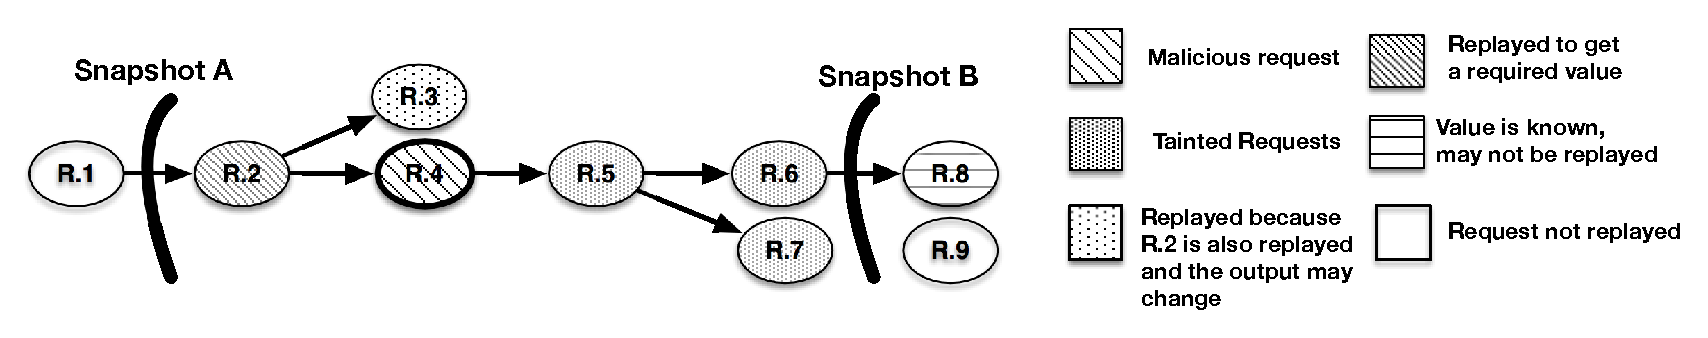
\includegraphics[width=150mm]{images/selectiveDependency_legended}
\caption[Dependency graph]{Dependency graph: $R.1$ is previous to a snapshot $A$; $R.3$ is dependent on $R.2$, which is replayed to get the read values; $R.4$ is a malicious request; $R.5,R.6,R.7$ are tainted; $R.8$ may not be replayed; $R.9$ is independent of the rest}
\label{fig:selectiveGraph}
\end{figure}

The selective replay process is as follows (full replay is simpler so we skip it):
\begin{enumerate}
\item \textit{Determine the malicious requests $A_{intrusion}$.}
Based on initial data such as user session compromised or data items accessed or other criteria, the tenant determines the requests $A_{intrusion}$ used by the attacker to compromise the application. For instance, $A_{intrusion} = \{R.4\} $ in Figure \ref{fig:selectiveGraph}.

\item \textit{Use $A_{intrusion}$ to determine the set of tainted requests $A_{tainted}$.}
For each request in $A_{intrusion}$, traverse the dependency graph in causality order and add these nodes to $A_{tainted}$ (in the figure $A_{tainted} = \{R.5,R.6,R.7,R.8\}$).


\item \textit{Get the requests needed to obtain the values read by $A_{tainted}$ and their effects.} 
Instead of storing the input and output of every action or versions of every data item, we propose to replay the actions which $A_{tainted}$ depends on. The data item value is known at the snapshot instant so the algorithm transverses the graph in inverse causality order from each request in $A_{tainted}$ and stores the requests in $A_{replay}$ ($A_{replay} = \{R.2\} \cup A_{tainted}$). $A_{replay}$ is expanded by traversing the graph from each of its elements on causality order to determine the requests which can be affected by the re-execution of $A_{replay}$ ($A_{replay} = A_{replay} \cup R.3$). Requests subsequent to the first snapshot after the latest malicious request may not be repeated as the data item version is known (version read by $R.8$ is stored in snapshot B).

\item \textit{Determine the replay order.} 
The set $A_{replay}$ is sorted on non-clustered \emph{start-end order}.

\item \textit{Load the previous data item versions}
Shuttle loads the version in the selected snapshot of the data items read by the requests in $A_{replay}$ and written by $A_{malicious}$.

\item \textit{Replay the requests}
Requests in $A_{replay}$ are replayed. If an access is not contained in operation list, then a new dependency is established and the requests that accessed the data item during the first execution are also replayed as in \emph{taint propagation via replay} \cite{retro}. For instance, $R.9$ is replayed if it reads an item written during recovery process but not during normal execution. 
\end{enumerate}

%merging branches
%After replaying the tainted requests, Shuttle compares the branches. \hl{ver se isto é necessário, na prática pode carregar apenas os dados novos}
% Depois para fazer o merge: compara as branches indo de key em key e comparando o hash dos valores guardados. As combinações são:
% |  Old  |   Recuperada |
%    A            A           - (sao iguais) - está tudo bem, um algoritmo de compressão pode colocar ambas as versões a apontar para o mesmo valor
%    -            B           - (nova entrada) - A versão recuperada ganha
%    A            B           - (modificado) - A versão recuperada ganha

% As entradas recuperadas escrevem sobre as que existem. Neste caso, os items apagados são também apagados.


 %A eficacia e melhoramento do selective replay depende do numero de entradas afectadas. Um simulador foi implementado e os resultados sao apresentados nos testes.

 Shuttle does not require generating a dependency graph in non-clustered full replay mode. The dependency graph is required in the case of clustered full replay to identify the independent clusters of requests and on selective replay to determine the tainted requests. We use the database operation lists to create the dependency graph and to order the execution of parallel requests without knowledge of the application protocol. 
 
 In summary, the selective replay approach reduces the number of requests to be replayed during the recovery process but implies that the application remains unchanged and does not revert the actions performed by unlogged requests. 


%%%%%%%%%%%%%%%%%%%%%%%%%%%%%%%%%%%%%%%%%%%%%%%%%%%%%%%%%%%%%%%%%%%%%%%%%%%%%%%%%%%%%%%%%%%%%%%%%%%%%%%%%%%%%%%%%%%%%%%%%%%%
\section{Chapter Summary}
\label{sec:arch:summary}
Shuttle recovers from security intrusions loading a previous snapshot and replaying the legitimate requests. It uses database snapshot and clustering to reduce the recovery time. Shuttle leverages the pay-per-usage model of \ac{PaaS} to provide a cost-efficient and fast recovery service instantiating the replay instances and more application containers on demand during the recovery process. \\

Shuttle proposes two approaches to perform replay: selective replay and full replay. 

\begin{table}[h]
\centering
    \begin{tabular}{l|ll}
               & Clustering & Non-Clustering \\ \hline
    Selective &  \xmark     &  \cmark        \\
    Full      &  \cmark     &  \cmark             
    \end{tabular}
\caption{Shuttle Replay modes}
\label{tab:operation_types}
\end{table}

The full replay approach supports parallel re-execution of requests that belong to independent clusters (clustering). Clustering is not supported on selective replay because the \textit{taint propagation via replay} defines the set of requests to replay at running time. Clustering is not supported with selective replay because taint propagation via replay defines the set of requests to be replayed in runtime.

The decentralized applications are more vulnerable to failures because of the single proxy architecture. However, we argue that future architectures can consider replication of the proxy, load balancer, Shuttle Storage and database. 
%!TEX encoding = UTF-8 Unicode
%!TEX root = ../paper.tex
\section{Recovery}
\label{sec:recovery}

Tenants initiate a recovery when they detect intrusions. When Shuttle enters recovery mode, it generates a list of requests to replay and asks for the \ac{PaaS} controller to launch a set of \textit{replay instances}. Shuttle may also ask for additional database and application server instances, or they may be launched automatically by the \ac{PaaS} platform when it detects additional load, in case auto-scaling is supported. The non-tampered snapshot that precedes the intrusion instant is selected. The multi-thread HTTP client of each replay instance fetches requests from \emph{Shuttle Storage} and sends them to the application servers, concurrently whenever possible. After replaying all requests issued before the beginning of the recovery, the manager sets the proxy state to \emph{restraining mode} and commands the replay instances to reexecute the remaining requests (those issued after recovery began). Then, \emph{restraining mode} is disabled. 
The following sections explain this process in detail.


%%%%%%%%%%%%%%%%%%%%%%%%%%%%%%%%%%%%%%%%%%%%%%%%%%%%%%%%%%%%%%%%%%%%%%%%%%%%%%%%%%%%%%%%%%%%%%%%%%%%%%%%%%%%%%%%%%%%%%%%%%%%%%
\subsection{Intrusion Identification}
\label{sec:recovery:detection}

%how the damage is fixed?
The recovery process starts when an intrusion is detected.\footnote{The way in which this detection is specifically done is out of the scope of the work  as we focus on recovery, not detection.} Intrusions may tamper the database \LONG{, e.g., modifying data,}or the application server instances\LONG{, e.g., changing the code of the application}. In order to fix the vulnerabilities that may have lead to intrusions, Shuttle supports the following actions: 1) update the application software; 2) identify a set of tampered database items; 3) add, modify or remove logged requests; 4) launch cleaned database and application server instances.

If tenants update the application software, they have to ensure that the application's interface remains compatible with the requests that will be replayed. If the database is tampered using user requests,  tenants have to identify the malicious user requests. For instance, a tenant can provide the set of suspicious database items to Shuttle and it will resolve the set of requests that accessed the suspicious items after the estimated intrusion moment. Knowing the suspicious requests, the tenant shall use Shuttle to add, modify or remove the past accidental or malicious requests. 

%%%%%%%%%%%%%%%%%%%%%%%%%%%%%%%%%%%%%%%%%%%%%%%%%%%%%%%%%%%%%%%%%%%%%%%%%%%%%%%%%%%%%%%%%%%%%%%%%%%%%%%%%%%%%%%%%%%%%%%%%%%%%
\subsection{Dependency graph}
\label{sec:recovery:dependencies}

%What is it? how it is generated?
A \emph{dependency graph} consists of nodes that represent requests and edges that establish dependencies between them (Figure \ref{fig:selectiveGraph}). Dependencies between requests are established using the following rules: 1) a request $R_A$ is dependent upon request $R_B$ if there is a data item $x$ such that $R_A$ read $x$ and $R_B$ performed the latest update on $x$; 2) dependencies are transitive except when requests perform blind writes (i.e., when requests write items without reading them first \cite{itdb}). \LONG{cite{Ammann2002}}

Previous solutions for relational databases extract the dependencies using a pre-defined, manually-created, per-transaction type template \cite{itdb}\LONG{cite{Ammann2002}}, or change the relational database management system code to extract read dependencies \cite{phoenix}. In contrast, Shuttle uses the database proxy to log the database accesses. Periodically, each database proxy traverses, in background, the \emph{operation list} of each data item to collect the new accesses and to generate the dependencies between requests. The Shuttle manager processes the dependencies to update the dependency graph. An alternative approach is to pull the dependencies from each database node only before the recovery process and generate the dependency graph when needed. The dependency graph is implemented as a hash table. The keys of the hash table are the \ac{RID}. Each value of the hash table contains the requests that depend on the associated request, i.e., the requests that execute after this one. A scalable implementation can use a distributed hash table or a graph-oriented database.
%type template: Um template que é pré-definido para cada transacção possivel. Na prática, deve ser uma classe para cada tipo de transacção que faz parsing da transacção para conseguir perceber que entradas é que vai ler ou escrever.

%false positives: detected but not exist
The above method may lead to \emph{false positives}, i.e., to flag dependencies that do not exist. For instance, a request may read a data item but not use it to compute the written value, so there is no real dependency. Although tracking variables used by each request during its execution might solve this particular case \cite{Akkus2010}, it would require modifying the code interpreter (e.g., Zend Engine for PHP), which would constrain Shuttle to a set of specific languages. As our approach uses dependencies just to group the requests that can be executed concurrently, false dependencies imply a performance penalty but do not cause data loss or inconsistent state.

%false negatives: not detected but exist
Complex queries on a relational database may lead to \emph{false negatives}, for instance when a read operation would have been executed on a deleted data item if this data item had not been deleted before the request execution \cite{Xie2008}. In contrast with SQL queries that access the data items that match a query, the \ac{CRUD} interface of most key-value stores specifies, in a deterministic and apriori manner, the data item that will be accessed. Shuttle logs every access, even when the data items do not exist, keeping the \emph{operation list} of the deleted data items to track further operations.


%%%%%%%%%%%%%%%%%%%%%%%%%%%%%%%%%%%%%%%%%%%%%%%%%%%%%%%%%%%%%%%%%%%%%%%%%%%%%%%%%%%%%%%%%%%%%%%%%%%%%%%%%%%%%%%%%%%%%%%%%%%%%%
\subsection{Replay}
\label{sec:recovery:replay}

Shuttle aims to support a large range of applications in which the user requests access a distributed database without using transactions. This assumption contrasts with previous recovery systems that set the order of requests based on the semantics of the application they consider (e.g., \cite{undoForOperators}) or the serialization provided by snapshot isolation (e.g., \cite{Akkus2010}). Moreover, requests executed concurrently during  normal execution, may  depend on each other (e.g., the first reads an item written by the second and the second reads an item written by the first).

%how I sort the requests?
We propose a new approach to order the requests for replaying that consists on sorting the requests per \emph{start-end order}, instead of using a dependency graph. Requests are replayed ordered by their start instant. Moreover, if a request starts before the end of another request, then they were executed concurrently and they are also re-executed concurrently. 
%DB Ordering
Yet, re-execution of concurrent requests is not deterministic, e.g., due to multi-thread servers, messaging systems, etc. Therefore our novel approach uses the \emph{operation list} to make parallel replay deterministic, by forcing operations on a data item during replay to follow the order established by its operation list (Figure \ref{fig:inconsistency_db_order}).

%locked requests
Modifications to the application code or to the sequence of requests may cause the application not to access the same sequence of data items or read/write the same content during the replay phase (Figure \ref{fig:inconsistency_unlock}). If an operation contained in the operation list is not performed, the following operations to the data item are blocked. To address this problem, at the end of each request execution, the \textit{interceptor} fetches the list of data items accessed by the request on its first execution and compares them against the ones accessed during the replay process. The database client library invokes the \emph{database proxy} with the keys that have not been accessed to unlock the remaining requests. 


\begin{figure*}[!thp]
  \centering
  \mbox{
          \subfloat[][Ordered by operation list \label{fig:inconsistency_db_order}]{
              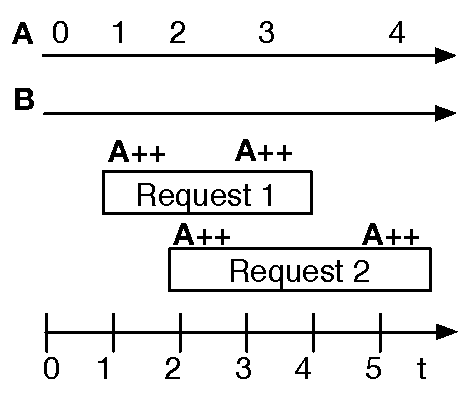
\includegraphics[width=0.17\linewidth]{images/inconsistency_db_order}
          }

          \subfloat[][Operation unlock \label{fig:inconsistency_unlock}]{
              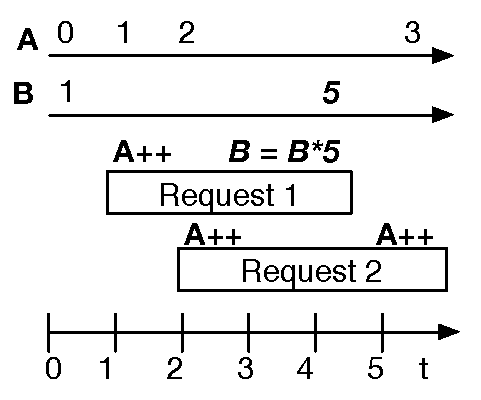
\includegraphics[width=0.17\linewidth]{images/inconsistency_unlock}
          }

          \subfloat[][Consecutive requests \label{fig:inconsistency_serial}]{
              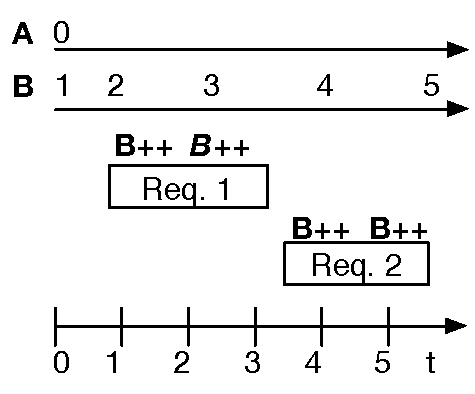
\includegraphics[width=0.17\linewidth]{images/inconsistency_serial}
          }

          \subfloat[][Conflict \label{fig:inconsistency_conflict}]{
              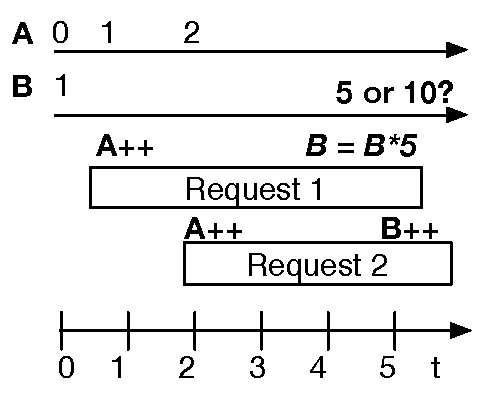
\includegraphics[width=0.17\linewidth]{images/inconsistency_conflict}
          }
  }
  \caption{Different re-executions of two requests.}
  \label{fig:inconsistency}
  \vspace{-5mm}
\end{figure*}

During replay there may be non-deterministic situations, whenever an access is not contained in the operation list. Consider the case of Figure \ref{fig:inconsistency}. Figure \ref{fig:inconsistency_db_order} represents the first execution of two requests. During the recovery period, the intrusion was removed hence requests access different data items than in the first execution. If \emph{req.~2} started after the end of \emph{req.~1}, the replay would be consistent with the first execution (Figure \ref{fig:inconsistency_serial}). An approach using only the dependency graph would have inconsistent results because the new dependency happens at recovery time.


%Conflict 
The problematic scenario is two requests being executed concurrently in the original execution: the \emph{start-end order} defines that \emph{req.~1} and \emph{req.~2} are replayed concurrently (Figure \ref{fig:inconsistency_conflict}). The access to $A$ remains consistent with the first execution (\emph{req.~2} after \emph{req.~1}), since the accesses are constrained by the \emph{operation list} of $A$. However, the final value of $B$ is unpredictable because \emph{req.~1} may write $B$ before or after \emph{req.~2}. Since both requests did not access the data item $B$ during their execution, the operation list does not establish an access order. Therefore, the \emph{req.~1} and \emph{req.~2} may execute in a arbitrary order. The order of these requests is as deterministic as during the first execution: the operation of \emph{req.~1} can execute before, between or after \emph{req.~2}.

%versioning e conciliamento
In order to turn the replay process more consistent with the first execution, we leverage semantic reconciliation, as in Dynamo \cite{Decandia2007}. The case represented in Figure \ref{fig:inconsistency_conflict} is equivalent to a concurrent update, where two parallel writes are performed on distinct database instances. Each request writes a distinct version resulting in conflicting versions of an item. Developers use the application-assisted conflict resolution interface to merge the versions. In this case, the following read operation would access the values written by the latest operation. In Figure \ref{fig:inconsistency_conflict}, \emph{req.~2} could choose between $5$ and $1$.

%other sources of non-determinism - nao devia estar fora daqui?!
A related issue is the determinism of the application, i.e., the issue if two subsequent executions with the same initial state and requests can be guaranteed to have the same final state and outputs. In the general case, we want replay to produce the same state with the same requests, so applications shall be deterministic. 
Five of the main sources of non-determinism are: shared memory, thread concurrency, random number generation, timestamps, and message exchanging. We assume requests to be independent thus they do not share memory, and that concurrent threads are independent. The API provided by Shuttle provides deterministic random number generation and timestamps using the \ac{RID} as timestamp and pseudo-random number seed, so the replay of a request will use the same random numbers and timestamp (we consider a single timestamp per request to be enough for most applications). This mechanism is language independent. User requests and database accesses are ordered in a deterministic way using the operation list.


\subsection{Clustering}
\label{sec:recovery:clusters}

%Must execute some requests in parallel
%Our preliminary experiments have shown that replaying requests concurrently can reduce the recovery period. 
We want recovery to take a fraction of the time elapsed since the snapshot from which it starts (e.g., minutes). 
We address this problem by grouping  requests in \emph{clusters} that can be executed concurrently. 
A cluster is a set of requests that have dependencies between them but not from/to requests in other clusters. 

Clusters are created when the recovery is about to start by inspecting the dependency graph. Since clusters are independent, they can be executed concurrently by different \emph{replay instances} without  synchronization between them. Requests within the same cluster, are performed in start-end order (Section \ref{sec:recovery:replay}). Given that more requests are executed concurrently, Shuttle launches more application servers and database instances to process the replayed requests. Therefore, the replay phase throughput is bigger than during first execution and the recovery time is minimized. This mechanism requires that the dependencies remain unchanged during the recovery phase.
%, i.e,. all replayed operations are contained in the operation list but not all operations in the list must be replayed.


%%%%%%%%%%%%%%%%%%%%%%%%%%%%%%%%%%%%%%%%%%%%%%%%%%%%%%%%%%%%%%%%%%%%%%%%%%%%%%%%%%%%%%%%%%%%%%%%%%%%%%%%%%%%%%%%%%%%%%%%%%%%
\subsection{Full and Selective Replay}
\label{sec:recovery:selective_replay}

We propose two approaches for intrusion recovery: full replay and selective replay. Full replay consists in replaying every request done after the  snapshot. Executing many requests takes considerable time, so this approach is adequate for intrusions detected reasonably fast after they happen, e.g., a few days. Selective replay re-executes only part of the requests so it is faster than full-replay. However, it requires tenants to provide a set of malicious actions (i.e., requests) $A_{intrusion}$. This set is used to deduce the set of tainted requests $A_{tainted}$. A request is said to be tainted if it is one of the attacker’s requests or if it reads objects written by tainted request \cite{taser,itdb,phoenix}.  The selective replay process is as follows (full replay is simpler so we skip it):

{1)} \textit{Determine the malicious requests $A_{intrusion}$.}
  Based on initial data such as user session compromised or data items accessed, the tenant determines the requests $A_{intrusion}$ used by the attacker to compromise the application. For instance, $A_{intrusion} = \{R.4\} $ (Figure \ref{fig:selectiveGraph}).
  
{2)} \textit{Use $A_{intrusion}$ to determine the tainted requests $A_{tainted}$.}
  For each request in $A_{intrusion}$, traverse the dependency graph in causality order and add these nodes to $A_{tainted}$ (in the figure $A_{tainted} = \{R.5,R.6,R.7\}$).

{3)} \textit{Get the requests needed to obtain the values read by $A_{tainted}$.} %and their effects 
  Instead of storing the input and output of every action or versions of every data item, Shuttle replays the actions which $A_{tainted}$ depends on. The data item value is known at the snapshot instant so the algorithm transverses the graph in inverse causality order from each request in $A_{tainted}$ and stores the requests in $A_{replay}$ ($A_{replay} = \{R.2\} \cup A_{tainted}$). $A_{replay}$ is expanded by traversing the graph from each of its elements in causality order to determine the requests which can be affected by the re-execution of $A_{replay} = A_{replay} \cup \{R.3\}$. 
%Requests subsequent to the first snapshot after the latest malicious request may not be repeated if all their read operations read the value contained in the snapshot (version read by $R.8$ is stored in snapshot B).

{4)} \textit{Determine the replay order.} 
  The set $A_{replay}$ is sorted in \emph{start-end order} (no clustering possible).

{5)} \textit{Load the previous data item versions.}
  Loads the version in the selected snapshot of the data items read by the requests in $A_{replay}$ and written by $A_{malicious}$.

{6)} \textit{Replay the requests.}
  Requests in $A_{replay}$ are replayed. If an access is not contained in an operation list, then a new dependency is established and the requests that accessed the data item during the first execution are also replayed as in \cite{retro}. For instance, $R.9$ is replayed if it reads an item written during recovery process but not during normal execution. 

\begin{figure}
  \centering
  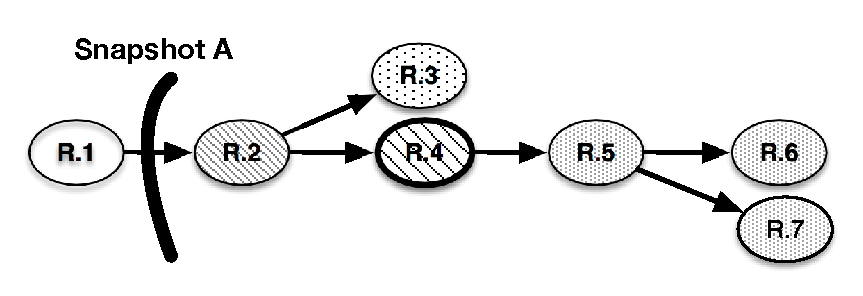
\includegraphics[width=0.7\linewidth]{images/selectiveDependency_paper}
  \caption{{Dependency graph:} $R.1$ precedes snapshot $A$; $R.3$ depends on $R.2$, which is replayed to get the read values; $R.4$ is a malicious request; $R.5,R.6,R.7$ are tainted.}
  \label{fig:selectiveGraph}
\end{figure}


%----------------------------------------------------------------------------------------------------------------------------
\subsection{Consistency}
\label{sec:recovery:consistency}

An important aspect of a recovery system like Shuttle is the application consistency seen by users. For instance, if a user does an action based on data written by a malicious action, which result of the user action replay is consistent? Since users have a non-deterministic behavior, they may have to be notified if a recovery took place and their data was modified.

Shuttle does not execute requests that returned an error in the first execution. Similarly to other works in the area \cite{undoForOperators}, we assume that these cases were compensated by the user when they happened. As only requests that did not return an error are replayed, Shuttle considers an inconsistency when a request returns an error or a response is different during replay. Shuttle provides the following API for the application programmer to define how inconsistencies are dealt with (Shuttle calls these functions in case they are defined by the tenant):

\begin{enumerate}
  \item \textit{preRecover():} invoked before the beginning of the recovery process.
  \item \textit{handleInconstency(request, previous response, new response, previous keys, new keys, action):} invoked when there is an inconsistency.
  \item \textit{postRecover(statistics, old version, new version):} invoked after the end of the recovery process.
\end{enumerate}

The first function allows tenants to perform a set of actions before the beginning of the recovery process, such as notifying the operations team or taking a new snapshot. 
The second function takes as input the operation that caused the inconsistency as well as the response and keys accessed during the normal execution and during the recovery process. It also takes as argument the action to take. Currently we consider three possible actions: 1) ignore the inconsistency; 2) notify the user of the inconsistency; 3) execute another request. 
Using the \textit{postRecover} function, the tenant has access not only to the statistics of the recovery process but also to an interface to compare the database values before and after the recovery process and the application responses, before exposing the data to the users. 

%mpc: isto faz sentido mas como nao se percebia nem qual era o problema nem o que o Shuttle fazia, preferi comentar
%Besides its users, an application may also interact with external services. \LONG{We simplify the problem by considering that applications only obtain inputs from external services, disregarding the issue of outputs.}The problem is treated in \cite{aire,undoForOperators}. 



%%%%%%%%%%%%%%%%%%%%%%%%%%%%%%%%%%%%%%%%%%%%%%%%%%%%%%%%%%%%%%%%%%%%%%%%%%%%%%%%%%%%%%%%%%%%%%%%%%%%%%%%%%%%%%%%%%%%%%%%%%%%%%
\subsection{Instance Rejuvenation}
\label{sec:recovery:instance_rejuventaion}
% Why? Because the instances can be corrupted
Attackers may exploit system vulnerabilities to tamper application server or database instances, affecting the application integrity or availability. Shuttle interacts with the \ac{PaaS} controller to rejuvenate instances when they are compromised. This process terminates the instances and launches new ones. The PaaS controller initializes the new instances with updated machine images and deploys an updated version of the application code, which may include updates to fix discovered flaws or prevent future intrusions.

We assume new instances to be intrusion-free as the image can be updated to fix previous flaws and their persistent state is renewed. Instances can be launched in a remote site to recover from catastrophic disasters \cite{cloud-disaster}. Tenants are responsible for ensuring that request dependencies remain correct and the updated version API is compatible, or for providing a script to update each request to the new API. Moreover, the selected snapshot has to be consistent according to the updated version specification or every request executed since the application's begin shall be replayed.
%mpc: "Instances can be launched in a remote site to recover from catastrophic disasters" ??

This process can be used in a proactive manner to renew instances to remove unknown intrusions \LONG{cite{Castro2002}}\cite{Sousa2010} or to test new application versions to compare its results against the previous version, using the branching mechanism (Section \ref{sec:recovery:runtime_recovery}).


%%%%%%%%%%%%%%%%%%%%%%%%%%%%%%%%%%%%%%%%%%%%%%%%%%%%%%%%%%%%%%%%%%%%%%%%%%%%%%%%%%%%%%%%%%%%%%%%%%%%%%%%%%%%%%%%%%%%%%%%%%%%%%
\subsection{Recovery in Runtime}
\label{sec:recovery:runtime_recovery}
%why?
Shuttle is capable of doing recovery in runtime, i.e., without making the application unavailable during the recovery period. To do so, each recovery process is considered to be a new branch, a model inspired in versioning systems such as \emph{git} \cite{git}. A \emph{branch} is a sequence of snapshots (akin to commits in \emph{git}). Figure \ref{fig:branches} presents an example with 2 branches and 4 snapshots.

\begin{SCfigure}
  \centering
  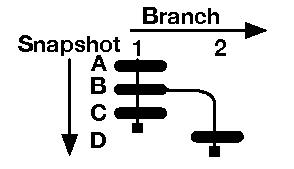
\includegraphics[width=30mm]{images/branches_paper}
  \caption{\footnotesize{Tree model:} 2 branches and 4 snapshots: branch 1 contains snapshots A,B,C; Branch 2 contains snapshots A,B,D.} %;\newline Branch 3 contains E.}
  \label{fig:branches}
\end{SCfigure}

Each recovery process creates a new branch forking a previous snapshot chosen by the tenant, either explicitly or implicitly (by indicating the initial intrusion instant, selecting implicitly the preceding snapshot). Incoming user requests access only the data of the previous branch keeping the application available, while replayed requests access the created branch without compromising the availability of the application. In addiction, tenants can use the branching mechanism to test their intrusion recovery procedures in background, i.e, without exposing users to test issues.

%branch-path
Since tenants can select previous snapshots, we define a branch as a sequence of non-tampered snapshots, named \emph{branch path}. For instance, the snapshots $A,B,D$ compose  branch 2 in the figure. Every database instance knows the \emph{branch path} of the previous branch and the newly created branch in use by the requests being replayed.

%How it works? 
Since a novel data item version is created only when the data item is written for the first time during each snapshot, the data item may not have a version for each snapshot (Section \ref{sec:architecture:snapshot}). Therefore, the version accessed by an operation is defined using the branch path and the \emph{version list} of the data item: operations read the latest version present in the \emph{version list} and in the \emph{branch path} and write the latest version in the branch path. A new version is added to the version list on the first access to each data item during the replay. This mechanism allows mapping the request to the correct version. Since the \emph{version list} keeps a pointer to the latest version and this reference is updated, the complexity of getting the correct version is $O(1)$. 

%Working explanation
At recovery time, the manager sends the new \emph{branch path} to every database instance. The new incoming users access the, perhaps corrupted, old branch while the requests being replaced access the new branch. Therefore, the application remains online, perhaps with a degraded behavior, without exposing downtime to users.

At some point, when the recovery is finishing, the user requests have to start being issued to the new branch. To do so, after replaying the requests, the proxy flag \emph{restraining} is set and every new request is marked with the \emph{restrain} flag. Database accesses marked with \emph{restrain} are delayed. After replaying the requests retrieved during the recovery process, the proxy sets the new branch in the subfield \emph{branch} of \ac{SRD} of the new requests, the \emph{restrain} flag is disabled and the database nodes are notified to proceed the accesses. This mechanism delays the processing of some requests, but this has typically a duration of seconds, compared with a recovery process that may take many minutes or even hours.
%!TEX root = ../paper.tex
%!TEX encoding = UTF-8 Unicode

\section{Evaluation}
\label{sec:evaluation}

%mpc: que chatice: so' agora reparei que nao dizemos o numero de experiencias de cada tipo nem o desvio padrao ou similar (variancia, percentis) :-( 

In order to evaluate our approach, we integrated a Shuttle prototype with AppScale and Voldemort. AppScale \cite{Appscale} is an open-source version of Google App Engine. Voldemort \cite{Kreps} is an open source implementation of Dynamo \cite{Decandia2007}, developed and in use by LinkedIn. Shuttle’s prototype has been developed in Java (1400 lines of code for the proxy, 1800 for the manager, 300 for the interceptor, 900 for the replay instances and 1800 for the database proxy).


\subsection{Application Example: Ask}
\label{sec:evaluation:app}

To evaluate Shuttle we developed a \acf{QA} web application for \ac{PaaS} inspired on Stack Exchange\footnote{http://stackexchange.com} (1700 lines of code). The application represents a generic web application that accepts requests and stores the persistent state in  Voldemort. Its implementation is independent of Shuttle, i.e., Shuttle does not require the application to be modified. 

The application semantics implies the following dependencies: a) questions are independent among them; b) answers depend on previous answers and on votes to the same question; c) comments depend on the commented answer; d) votes depend on the answer they vote on. We selected subsets of a dump of the Stack Exchange database to simulate real-world requests.\footnote{Available at: https://archive.org/details/stackexchange} 

\subsection{Accuracy}
\label{sec:evaluation:accuracy}

We evaluate Shuttle's ability to correctly recover applications in different scenarios. We consider three classes of intrusion scenarios: malicious requests, software vulnerabilities and external channels (e.g., SSH connections). The selected data subset contains 100 000 requests originally performed from 31 July until 12 Sep.~2008: 6992 questions, 28993 answers, 2220 comments, 61795 votes. Requests were sorted per date, establishing 92 939 dependencies.

At intrusion moment, Sep.~2nd, the database contains 4338 questions, 18286 answers, 422 comments and 38334 votes (61380 requests). The attack is detected in Sep.~12th, assuming a pessimistic delay of 10 days. During this period, the application executed 38 620 requests. Table \ref{tab:accuracy} presents a summary of the accuracy tests. It contains the number of data items tampered by the intrusion (\emph{\#intrusion}) and the number of user requests that read data items written by  tainted requests or malicious requests (without considering the intrusion requests). Recovery using \textit{full replay} requires to replay every request from the latest snapshot before the intrusion instant until the detection instant: in this example at least 38 620 requests (\emph{\#replayed (fr)}). Selective replay only re-executes tainted requests, unless some data item versions need to be recreated. On the worst case, the system does not contain any snapshot and every data read by the tainted requests shall be recreated (\emph{\#replayed (sr)}). 

\begin{table}
\footnotesize
\begin{tabular}{l|rrrr}
    & \#intrusion & \#tainted & \#replayed (sr)     & \#replayed (fr) \\ \hline
1a       & 110          & 0          & $[0, 605]$   & $> 38 620$  \\
1b       & 58           & 14         & $[0, 379]$   & $> 38 620$  \\
1c       & 48           & 52         & $[0, 253]$   & $> 38 620$  \\
2a       & 4 338        & 0          &  -           & $> 38 620$  \\
2b       & 18 286       & 1 278      &  -           & $> 38 620$  \\
3        & 2 000        & -          &  -           & $> 38 620$  \\
\end{tabular}
  \caption{Number of requests replayed during the recovery process.}
  \label{tab:accuracy}
\end{table}

%Scenario A: tainted request
\textbf{Malicious Requests.} 
 In the first class of scenarios, we consider three cases in which an attacker has stolen an user credential, then: a) deleted every question created by the user; b) deleted every user answer; or c) modified every user answer.

\textit{1a)} The attacker deletes the user's 4 questions, performing 4 delete requests that remove 106 associated comments and answers. The tenant identifies the malicious requests through the user session and selects a snapshot previous to the intrusion instant. Users cannot access deleted questions, so no request is tainted. If Shuttle has a snapshot containing the deleted questions, then \textit{selective replay} does not need to replay any request and merges the deleted questions on the current system state. If the latest snapshot is previous to the creation of the 4 questions, then \textit{selective replay} replays 605 requests to recreate the deleted questions, their answers and votes. The result is merged with the current branch, rebuilding the deleted questions. 

\textit{1b)} Deleting the user's 48 answers implies that 58 data items are deleted and 14 answers and comments are tainted as they execute after the intrusion instant answering and voting without knowing some answers. If a snapshot containing the user answers exists, then the \textit{selective replay} approach replays only 14 tainted answers and comments. Otherwise, it replays 379 requests: the total number of requests to recreate the tainted questions and then merge the result.


\textit{1c)} 48 data items are modified while 52 requests are tainted because the users replays, votes and comments the modified questions after the intrusion instant. For recovery, the 52 tainted requests shall be replayed. If Shuttle does not have a snapshot containing the questions, then 253 requests have to be replayed to recreate them. 

\textbf{Software vulnerability.}
On the second class, we evaluate intrusion scenarios where software flaws allow attackers to modify the database without authorization. For instance, a code update added a flaw that allows SQL injection. We consider two independent scenarios where the attacker: a) deleted every question; b) deleted every answer.

In \textit{2a)}, the deleting of every question removes 4 338 data items. In \textit{2b)}, the questions are preserved but 1 278 answers, votes and comments are tainted as the user did not see the deleted answers.
%
Instead of identifying the requests that explored the vulnerability, the tenant patches the code to remove the application vulnerability. Tenants use the instance rejuvenation mechanism to shutdown current application containers and deploy new application version. After, they use the \textit{full replay} to repeat all requests since the beginning of usage of the software version with the flaw. Requests that explored the vulnerability fail to execute and a consistent application state is recovered.



\textbf{External channel.}
On the third class, we consider a case where the proxy does not log the attacker actions. The attacker might use, for example, a SSH account created exploiting the ShellShock vulnerability. The attacker stolen the database credentials and modified at least 2000 data items. Since these database operations are not logged, the dependencies are not established and the number of tainted requests is unknown. However, even without logging the malicious actions, Shuttle recovers the application by loading a database snapshot previous to the estimated intrusion instant (Sep.~2nd) and performing \textit{full replay}. The attack effects are removed because Shuttle loads a database snapshot instead of undoing every operation. As the malicious actions were not logged, they are not replayed and Shuttle recovers the application consistency.


The number of requests to replay is defined by the snapshot instant: on \textit{full replay} Shuttle replays all requests performed after the intrusion instant, while on \textit{selective replay} Shuttle replays the requests necessary to read the values of the entries before the intrusion and the tainted requests. While  \textit{selective replay} seems to have a big advantage comparing with  \textit{full replay}, which performs, in these scenarios, at least 38 620 requests, some applications have more dependencies thus the number of tainted requests is bigger. For instance, if the order between questions with the same tag is considered as a dependency, the number of dependencies rises from 92 939 to 109 118 and the number of independent clusters decreases from 6992 to 56. %We plan to further analyze the dependencies established by different applications. %mpc: o comentario estava ok mas como fomos criticados por a aplicacao poder nao ser representativa...



\subsection{Performance}
\label{sec:evaluation:performance}

We evaluate Shuttle's performance considering the throughput of the application, the size of the logs and the recovery time. We also estimate the cost of deployment of Shuttle on a public cloud provider, \acf{AWS}. We run 6 \ac{AWS} \textit{c3.xlarge} instances (14 ECUs, 4 vCPUs, 2.8 GHz, Intel Xeon E5-2680v2, 7.5 GB of memory, 2 x 40 GB storage capacity) connected by gigabit ethernet (780Mbps measured with \emph{iperf}, 0.176ms round-trip time measured with \emph{ping}). We use one client, one instance with Shuttle proxy and a load balancer (HAProxy), three WildFly (formerly JBoss) application servers and one Voldemort database. We consider a large data sample from the data of Stack Exchange with 50 000 requests (1432 questions, 3399 answers, 8335 comments, 36834 votes, 950 000 question views). We do not consider a particular scenario or replay scheme (full/selective), but define instead the number of requests recovered per experiment.

\textbf{Performance overhead.}
We evaluate the overhead of Shuttle by measuring the throughput of the \textit{Ask} application with and without Shuttle (Table \ref{tab:throughput}). We considered two workloads: (A) 50\% reads, 50\% writes;  (B)  95\% reads, 5\% writes. Write operations insert questions, answers, comments and votes of the data sample, while the read operations access the latest inserted questions. Table \ref{tab:throughput} shows that Shuttle imposes an overhead of 13-20\%, which seems reasonable considering its benefits. We believe the main cause of overhead is the current proxy implementation, which is not very efficient. The current version written in Java performs considerably better than a previous version in Python, but we expect to improve it further by rewriting it in C.

\begin{table}
\footnotesize
\begin{tabular}{l|rr}
                       &  Workload A                    & Workload B  \\ \hline
Shuttle                &  6325 ops/sec [5.78 ms]        &  15346 ops/sec [3.62 ms]  \\
No Shuttle             &  7148 ops/sec [5.07 ms]        &  17821 ops/sec [3.01 ms]  \\
overhead               &  13\% [14\%]                    & 16\% [20\%] \\
\end{tabular}
\caption{Overhead in throughput (ops/sec) and response latency (ms).}
\label{tab:throughput}
\end{table}

%\hl{estes resultados são estranhos, são tão bons quando comparados com os outros.}
%database overhead
In order to measure Shuttle's overhead on the database accesses, we used the \acf{YCSB} framework \cite{ycsb}. We considered two workloads: (A)  50\% reads, 50\% updates; (B)  95\% reads, 5\% updates. Operations access 1KB records following a Zipfian distribution (Figure \ref{fig:database_overhead}). Results show Shuttle has small impact on the latency of database accesses. 

\begin{figure}[tbh]
\vspace{-6mm}
\hspace*{-0.5cm}
  \LARGE
  \mbox{
      \subfloat[][Workload A - update \label{fig:database:a:update}]{
      \hspace{-0.5cm}
        \resizebox{4.5cm}{!}{% GNUPLOT: LaTeX picture with Postscript
\begingroup
  \makeatletter
  \providecommand\color[2][]{%
    \GenericError{(gnuplot) \space\space\space\@spaces}{%
      Package color not loaded in conjunction with
      terminal option `colourtext'%
    }{See the gnuplot documentation for explanation.%
    }{Either use 'blacktext' in gnuplot or load the package
      color.sty in LaTeX.}%
    \renewcommand\color[2][]{}%
  }%
  \providecommand\includegraphics[2][]{%
    \GenericError{(gnuplot) \space\space\space\@spaces}{%
      Package graphicx or graphics not loaded%
    }{See the gnuplot documentation for explanation.%
    }{The gnuplot epslatex terminal needs graphicx.sty or graphics.sty.}%
    \renewcommand\includegraphics[2][]{}%
  }%
  \providecommand\rotatebox[2]{#2}%
  \@ifundefined{ifGPcolor}{%
    \newif\ifGPcolor
    \GPcolorfalse
  }{}%
  \@ifundefined{ifGPblacktext}{%
    \newif\ifGPblacktext
    \GPblacktexttrue
  }{}%
  % define a \g@addto@macro without @ in the name:
  \let\gplgaddtomacro\g@addto@macro
  % define empty templates for all commands taking text:
  \gdef\gplbacktext{}%
  \gdef\gplfronttext{}%
  \makeatother
  \ifGPblacktext
    % no textcolor at all
    \def\colorrgb#1{}%
    \def\colorgray#1{}%
  \else
    % gray or color?
    \ifGPcolor
      \def\colorrgb#1{\color[rgb]{#1}}%
      \def\colorgray#1{\color[gray]{#1}}%
      \expandafter\def\csname LTw\endcsname{\color{white}}%
      \expandafter\def\csname LTb\endcsname{\color{black}}%
      \expandafter\def\csname LTa\endcsname{\color{black}}%
      \expandafter\def\csname LT0\endcsname{\color[rgb]{1,0,0}}%
      \expandafter\def\csname LT1\endcsname{\color[rgb]{0,1,0}}%
      \expandafter\def\csname LT2\endcsname{\color[rgb]{0,0,1}}%
      \expandafter\def\csname LT3\endcsname{\color[rgb]{1,0,1}}%
      \expandafter\def\csname LT4\endcsname{\color[rgb]{0,1,1}}%
      \expandafter\def\csname LT5\endcsname{\color[rgb]{1,1,0}}%
      \expandafter\def\csname LT6\endcsname{\color[rgb]{0,0,0}}%
      \expandafter\def\csname LT7\endcsname{\color[rgb]{1,0.3,0}}%
      \expandafter\def\csname LT8\endcsname{\color[rgb]{0.5,0.5,0.5}}%
    \else
      % gray
      \def\colorrgb#1{\color{black}}%
      \def\colorgray#1{\color[gray]{#1}}%
      \expandafter\def\csname LTw\endcsname{\color{white}}%
      \expandafter\def\csname LTb\endcsname{\color{black}}%
      \expandafter\def\csname LTa\endcsname{\color{black}}%
      \expandafter\def\csname LT0\endcsname{\color{black}}%
      \expandafter\def\csname LT1\endcsname{\color{black}}%
      \expandafter\def\csname LT2\endcsname{\color{black}}%
      \expandafter\def\csname LT3\endcsname{\color{black}}%
      \expandafter\def\csname LT4\endcsname{\color{black}}%
      \expandafter\def\csname LT5\endcsname{\color{black}}%
      \expandafter\def\csname LT6\endcsname{\color{black}}%
      \expandafter\def\csname LT7\endcsname{\color{black}}%
      \expandafter\def\csname LT8\endcsname{\color{black}}%
    \fi
  \fi
  \setlength{\unitlength}{0.0500bp}%
  \begin{picture}(7200.00,5040.00)%
    \gplgaddtomacro\gplbacktext{%
      \csname LTb\endcsname%
      \put(1078,704){\makebox(0,0)[r]{\strut{} 0}}%
      \put(1078,1629){\makebox(0,0)[r]{\strut{} 500}}%
      \put(1078,2554){\makebox(0,0)[r]{\strut{} 1000}}%
      \put(1078,3480){\makebox(0,0)[r]{\strut{} 1500}}%
      \put(1078,4405){\makebox(0,0)[r]{\strut{} 2000}}%
      \put(1210,484){\makebox(0,0){\strut{} 5}}%
      \put(2009,484){\makebox(0,0){\strut{} 10}}%
      \put(2808,484){\makebox(0,0){\strut{} 15}}%
      \put(3607,484){\makebox(0,0){\strut{} 20}}%
      \put(4406,484){\makebox(0,0){\strut{} 25}}%
      \put(5205,484){\makebox(0,0){\strut{} 30}}%
      \put(6004,484){\makebox(0,0){\strut{} 35}}%
      \put(6803,484){\makebox(0,0){\strut{} 40}}%
      \put(176,2739){\rotatebox{-270}{\makebox(0,0){\strut{}Update latency (us)}}}%
      \put(4006,154){\makebox(0,0){\strut{}Throughput (thousand ops/sec)}}%
    }%
    \gplgaddtomacro\gplfronttext{%
      \csname LTb\endcsname%
      \put(5816,1416){\makebox(0,0)[r]{\strut{}Shuttle}}%
      \csname LTb\endcsname%
      \put(5816,1042){\makebox(0,0)[r]{\strut{}No Shuttle}}%
    }%
    \gplbacktext
    \put(0,0){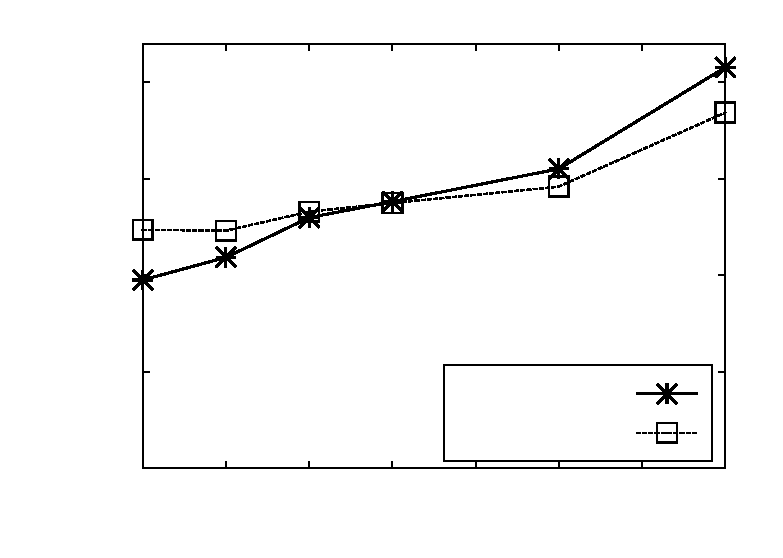
\includegraphics{graphs/database/a_update}}%
    \gplfronttext
  \end{picture}%
\endgroup
}
      }
      \subfloat[][Workload B - read \label{fig:database:b:read}]{
      \hspace{-0.7cm}
        \resizebox{4.5cm}{!}{% GNUPLOT: LaTeX picture with Postscript
\begingroup
  \makeatletter
  \providecommand\color[2][]{%
    \GenericError{(gnuplot) \space\space\space\@spaces}{%
      Package color not loaded in conjunction with
      terminal option `colourtext'%
    }{See the gnuplot documentation for explanation.%
    }{Either use 'blacktext' in gnuplot or load the package
      color.sty in LaTeX.}%
    \renewcommand\color[2][]{}%
  }%
  \providecommand\includegraphics[2][]{%
    \GenericError{(gnuplot) \space\space\space\@spaces}{%
      Package graphicx or graphics not loaded%
    }{See the gnuplot documentation for explanation.%
    }{The gnuplot epslatex terminal needs graphicx.sty or graphics.sty.}%
    \renewcommand\includegraphics[2][]{}%
  }%
  \providecommand\rotatebox[2]{#2}%
  \@ifundefined{ifGPcolor}{%
    \newif\ifGPcolor
    \GPcolorfalse
  }{}%
  \@ifundefined{ifGPblacktext}{%
    \newif\ifGPblacktext
    \GPblacktexttrue
  }{}%
  % define a \g@addto@macro without @ in the name:
  \let\gplgaddtomacro\g@addto@macro
  % define empty templates for all commands taking text:
  \gdef\gplbacktext{}%
  \gdef\gplfronttext{}%
  \makeatother
  \ifGPblacktext
    % no textcolor at all
    \def\colorrgb#1{}%
    \def\colorgray#1{}%
  \else
    % gray or color?
    \ifGPcolor
      \def\colorrgb#1{\color[rgb]{#1}}%
      \def\colorgray#1{\color[gray]{#1}}%
      \expandafter\def\csname LTw\endcsname{\color{white}}%
      \expandafter\def\csname LTb\endcsname{\color{black}}%
      \expandafter\def\csname LTa\endcsname{\color{black}}%
      \expandafter\def\csname LT0\endcsname{\color[rgb]{1,0,0}}%
      \expandafter\def\csname LT1\endcsname{\color[rgb]{0,1,0}}%
      \expandafter\def\csname LT2\endcsname{\color[rgb]{0,0,1}}%
      \expandafter\def\csname LT3\endcsname{\color[rgb]{1,0,1}}%
      \expandafter\def\csname LT4\endcsname{\color[rgb]{0,1,1}}%
      \expandafter\def\csname LT5\endcsname{\color[rgb]{1,1,0}}%
      \expandafter\def\csname LT6\endcsname{\color[rgb]{0,0,0}}%
      \expandafter\def\csname LT7\endcsname{\color[rgb]{1,0.3,0}}%
      \expandafter\def\csname LT8\endcsname{\color[rgb]{0.5,0.5,0.5}}%
    \else
      % gray
      \def\colorrgb#1{\color{black}}%
      \def\colorgray#1{\color[gray]{#1}}%
      \expandafter\def\csname LTw\endcsname{\color{white}}%
      \expandafter\def\csname LTb\endcsname{\color{black}}%
      \expandafter\def\csname LTa\endcsname{\color{black}}%
      \expandafter\def\csname LT0\endcsname{\color{black}}%
      \expandafter\def\csname LT1\endcsname{\color{black}}%
      \expandafter\def\csname LT2\endcsname{\color{black}}%
      \expandafter\def\csname LT3\endcsname{\color{black}}%
      \expandafter\def\csname LT4\endcsname{\color{black}}%
      \expandafter\def\csname LT5\endcsname{\color{black}}%
      \expandafter\def\csname LT6\endcsname{\color{black}}%
      \expandafter\def\csname LT7\endcsname{\color{black}}%
      \expandafter\def\csname LT8\endcsname{\color{black}}%
    \fi
  \fi
  \setlength{\unitlength}{0.0500bp}%
  \begin{picture}(7200.00,5040.00)%
    \gplgaddtomacro\gplbacktext{%
      \csname LTb\endcsname%
      \put(1078,704){\makebox(0,0)[r]{\strut{} 0}}%
      \put(1078,1629){\makebox(0,0)[r]{\strut{} 500}}%
      \put(1078,2554){\makebox(0,0)[r]{\strut{} 1000}}%
      \put(1078,3480){\makebox(0,0)[r]{\strut{} 1500}}%
      \put(1078,4405){\makebox(0,0)[r]{\strut{} 2000}}%
      \put(1210,484){\makebox(0,0){\strut{} 5}}%
      \put(2009,484){\makebox(0,0){\strut{} 10}}%
      \put(2808,484){\makebox(0,0){\strut{} 15}}%
      \put(3607,484){\makebox(0,0){\strut{} 20}}%
      \put(4406,484){\makebox(0,0){\strut{} 25}}%
      \put(5205,484){\makebox(0,0){\strut{} 30}}%
      \put(6004,484){\makebox(0,0){\strut{} 35}}%
      \put(6803,484){\makebox(0,0){\strut{} 40}}%
      \put(176,2739){\rotatebox{-270}{\makebox(0,0){\strut{}Read latency (us)}}}%
      \put(4006,154){\makebox(0,0){\strut{}Throughput (thousand ops/sec)}}%
    }%
    \gplgaddtomacro\gplfronttext{%
      \csname LTb\endcsname%
      \put(5816,1416){\makebox(0,0)[r]{\strut{}Shuttle}}%
      \csname LTb\endcsname%
      \put(5816,1042){\makebox(0,0)[r]{\strut{}No Shuttle}}%
    }%
    \gplbacktext
    \put(0,0){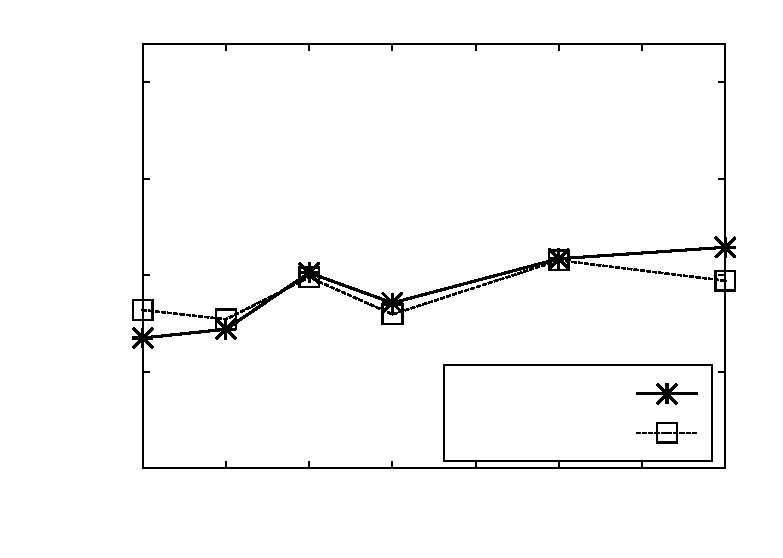
\includegraphics{graphs/database/b_read}}%
    \gplfronttext
  \end{picture}%
\endgroup
}
      }
  }
  \caption{Performance overhead on database.}
  \vspace{-2mm}
  \label{fig:database_overhead}
\end{figure}


\textbf{Recovery.}
We measured the recovery time using Shuttle to replay the sample of 1 million requests. While serial replay (1 cluster) takes approximately 30 minutes (1717s), recovery with clusters takes only 9 minutes (544s) (Figure \ref{fig:recovery_times}).

We measured the recovery period with different numbers of instances on clustered mode (Figure \ref{fig:scalability}). The figure shows that Shuttle is scalable, in the sense that adding more servers allow reducing the time of recovery (3 servers allowed recovery in half the time of 1, $\sim$750s versus $\sim$400s). 

%Shuttle scalability: Recovery time considering the number of database and web-server instances and the number of acting users in parallel (runtime-recovery). On clustered mode, each cluster is replayed by one replay instance.
\begin{figure}[tbh]
\vspace{-5mm}
  \LARGE
  \mbox{
      \subfloat[][Recovery time \label{fig:recovery_times}]{
      \hspace{-0.5cm}
        \resizebox{4.5cm}{!}{% GNUPLOT: LaTeX picture with Postscript
\begingroup
  \makeatletter
  \providecommand\color[2][]{%
    \GenericError{(gnuplot) \space\space\space\@spaces}{%
      Package color not loaded in conjunction with
      terminal option `colourtext'%
    }{See the gnuplot documentation for explanation.%
    }{Either use 'blacktext' in gnuplot or load the package
      color.sty in LaTeX.}%
    \renewcommand\color[2][]{}%
  }%
  \providecommand\includegraphics[2][]{%
    \GenericError{(gnuplot) \space\space\space\@spaces}{%
      Package graphicx or graphics not loaded%
    }{See the gnuplot documentation for explanation.%
    }{The gnuplot epslatex terminal needs graphicx.sty or graphics.sty.}%
    \renewcommand\includegraphics[2][]{}%
  }%
  \providecommand\rotatebox[2]{#2}%
  \@ifundefined{ifGPcolor}{%
    \newif\ifGPcolor
    \GPcolorfalse
  }{}%
  \@ifundefined{ifGPblacktext}{%
    \newif\ifGPblacktext
    \GPblacktexttrue
  }{}%
  % define a \g@addto@macro without @ in the name:
  \let\gplgaddtomacro\g@addto@macro
  % define empty templates for all commands taking text:
  \gdef\gplbacktext{}%
  \gdef\gplfronttext{}%
  \makeatother
  \ifGPblacktext
    % no textcolor at all
    \def\colorrgb#1{}%
    \def\colorgray#1{}%
  \else
    % gray or color?
    \ifGPcolor
      \def\colorrgb#1{\color[rgb]{#1}}%
      \def\colorgray#1{\color[gray]{#1}}%
      \expandafter\def\csname LTw\endcsname{\color{white}}%
      \expandafter\def\csname LTb\endcsname{\color{black}}%
      \expandafter\def\csname LTa\endcsname{\color{black}}%
      \expandafter\def\csname LT0\endcsname{\color[rgb]{1,0,0}}%
      \expandafter\def\csname LT1\endcsname{\color[rgb]{0,1,0}}%
      \expandafter\def\csname LT2\endcsname{\color[rgb]{0,0,1}}%
      \expandafter\def\csname LT3\endcsname{\color[rgb]{1,0,1}}%
      \expandafter\def\csname LT4\endcsname{\color[rgb]{0,1,1}}%
      \expandafter\def\csname LT5\endcsname{\color[rgb]{1,1,0}}%
      \expandafter\def\csname LT6\endcsname{\color[rgb]{0,0,0}}%
      \expandafter\def\csname LT7\endcsname{\color[rgb]{1,0.3,0}}%
      \expandafter\def\csname LT8\endcsname{\color[rgb]{0.5,0.5,0.5}}%
    \else
      % gray
      \def\colorrgb#1{\color{black}}%
      \def\colorgray#1{\color[gray]{#1}}%
      \expandafter\def\csname LTw\endcsname{\color{white}}%
      \expandafter\def\csname LTb\endcsname{\color{black}}%
      \expandafter\def\csname LTa\endcsname{\color{black}}%
      \expandafter\def\csname LT0\endcsname{\color{black}}%
      \expandafter\def\csname LT1\endcsname{\color{black}}%
      \expandafter\def\csname LT2\endcsname{\color{black}}%
      \expandafter\def\csname LT3\endcsname{\color{black}}%
      \expandafter\def\csname LT4\endcsname{\color{black}}%
      \expandafter\def\csname LT5\endcsname{\color{black}}%
      \expandafter\def\csname LT6\endcsname{\color{black}}%
      \expandafter\def\csname LT7\endcsname{\color{black}}%
      \expandafter\def\csname LT8\endcsname{\color{black}}%
    \fi
  \fi
  \setlength{\unitlength}{0.0500bp}%
  \begin{picture}(7200.00,5040.00)%
    \gplgaddtomacro\gplbacktext{%
      \csname LTb\endcsname%
      \put(1078,704){\makebox(0,0)[r]{\strut{} 0}}%
      \put(1078,1518){\makebox(0,0)[r]{\strut{} 500}}%
      \put(1078,2332){\makebox(0,0)[r]{\strut{} 1000}}%
      \put(1078,3147){\makebox(0,0)[r]{\strut{} 1500}}%
      \put(1078,3961){\makebox(0,0)[r]{\strut{} 2000}}%
      \put(1078,4775){\makebox(0,0)[r]{\strut{} 2500}}%
      \put(1210,484){\makebox(0,0){\strut{}00:00}}%
      \put(2142,484){\makebox(0,0){\strut{}05:00}}%
      \put(3074,484){\makebox(0,0){\strut{}10:00}}%
      \put(4007,484){\makebox(0,0){\strut{}15:00}}%
      \put(4939,484){\makebox(0,0){\strut{}20:00}}%
      \put(5871,484){\makebox(0,0){\strut{}25:00}}%
      \put(6803,484){\makebox(0,0){\strut{}30:00}}%
      \put(176,2739){\rotatebox{-270}{\makebox(0,0){\strut{}Requests per second}}}%
      \put(4006,154){\makebox(0,0){\strut{}Time (minutes:seconds)}}%
    }%
    \gplgaddtomacro\gplfronttext{%
      \csname LTb\endcsname%
      \put(5816,4481){\makebox(0,0)[r]{\strut{}serial replay}}%
      \csname LTb\endcsname%
      \put(5816,4195){\makebox(0,0)[r]{\strut{}clustered replay}}%
    }%
    \gplbacktext
    \put(0,0){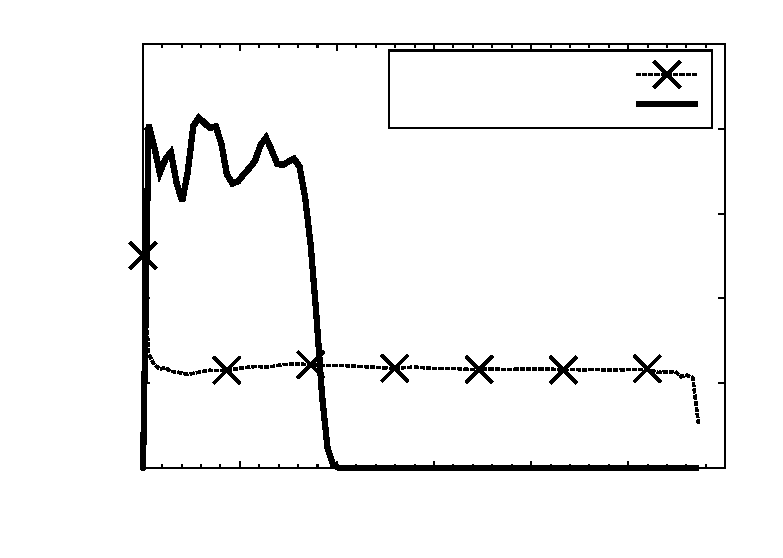
\includegraphics{graphs/replay/grafico_paper}}%
    \gplfronttext
  \end{picture}%
\endgroup
}
      }
      \subfloat[][Scalability \label{fig:scalability}]{
      \hspace{-0.7cm}
        \resizebox{4.5cm}{!}{% GNUPLOT: LaTeX picture with Postscript
\begingroup
  \makeatletter
  \providecommand\color[2][]{%
    \GenericError{(gnuplot) \space\space\space\@spaces}{%
      Package color not loaded in conjunction with
      terminal option `colourtext'%
    }{See the gnuplot documentation for explanation.%
    }{Either use 'blacktext' in gnuplot or load the package
      color.sty in LaTeX.}%
    \renewcommand\color[2][]{}%
  }%
  \providecommand\includegraphics[2][]{%
    \GenericError{(gnuplot) \space\space\space\@spaces}{%
      Package graphicx or graphics not loaded%
    }{See the gnuplot documentation for explanation.%
    }{The gnuplot epslatex terminal needs graphicx.sty or graphics.sty.}%
    \renewcommand\includegraphics[2][]{}%
  }%
  \providecommand\rotatebox[2]{#2}%
  \@ifundefined{ifGPcolor}{%
    \newif\ifGPcolor
    \GPcolorfalse
  }{}%
  \@ifundefined{ifGPblacktext}{%
    \newif\ifGPblacktext
    \GPblacktexttrue
  }{}%
  % define a \g@addto@macro without @ in the name:
  \let\gplgaddtomacro\g@addto@macro
  % define empty templates for all commands taking text:
  \gdef\gplbacktext{}%
  \gdef\gplfronttext{}%
  \makeatother
  \ifGPblacktext
    % no textcolor at all
    \def\colorrgb#1{}%
    \def\colorgray#1{}%
  \else
    % gray or color?
    \ifGPcolor
      \def\colorrgb#1{\color[rgb]{#1}}%
      \def\colorgray#1{\color[gray]{#1}}%
      \expandafter\def\csname LTw\endcsname{\color{white}}%
      \expandafter\def\csname LTb\endcsname{\color{black}}%
      \expandafter\def\csname LTa\endcsname{\color{black}}%
      \expandafter\def\csname LT0\endcsname{\color[rgb]{1,0,0}}%
      \expandafter\def\csname LT1\endcsname{\color[rgb]{0,1,0}}%
      \expandafter\def\csname LT2\endcsname{\color[rgb]{0,0,1}}%
      \expandafter\def\csname LT3\endcsname{\color[rgb]{1,0,1}}%
      \expandafter\def\csname LT4\endcsname{\color[rgb]{0,1,1}}%
      \expandafter\def\csname LT5\endcsname{\color[rgb]{1,1,0}}%
      \expandafter\def\csname LT6\endcsname{\color[rgb]{0,0,0}}%
      \expandafter\def\csname LT7\endcsname{\color[rgb]{1,0.3,0}}%
      \expandafter\def\csname LT8\endcsname{\color[rgb]{0.5,0.5,0.5}}%
    \else
      % gray
      \def\colorrgb#1{\color{black}}%
      \def\colorgray#1{\color[gray]{#1}}%
      \expandafter\def\csname LTw\endcsname{\color{white}}%
      \expandafter\def\csname LTb\endcsname{\color{black}}%
      \expandafter\def\csname LTa\endcsname{\color{black}}%
      \expandafter\def\csname LT0\endcsname{\color{black}}%
      \expandafter\def\csname LT1\endcsname{\color{black}}%
      \expandafter\def\csname LT2\endcsname{\color{black}}%
      \expandafter\def\csname LT3\endcsname{\color{black}}%
      \expandafter\def\csname LT4\endcsname{\color{black}}%
      \expandafter\def\csname LT5\endcsname{\color{black}}%
      \expandafter\def\csname LT6\endcsname{\color{black}}%
      \expandafter\def\csname LT7\endcsname{\color{black}}%
      \expandafter\def\csname LT8\endcsname{\color{black}}%
    \fi
  \fi
  \setlength{\unitlength}{0.0500bp}%
  \begin{picture}(7200.00,5040.00)%
    \gplgaddtomacro\gplbacktext{%
      \csname LTb\endcsname%
      \put(946,704){\makebox(0,0)[r]{\strut{} 0}}%
      \put(946,1156){\makebox(0,0)[r]{\strut{} 100}}%
      \put(946,1609){\makebox(0,0)[r]{\strut{} 200}}%
      \put(946,2061){\makebox(0,0)[r]{\strut{} 300}}%
      \put(946,2513){\makebox(0,0)[r]{\strut{} 400}}%
      \put(946,2966){\makebox(0,0)[r]{\strut{} 500}}%
      \put(946,3418){\makebox(0,0)[r]{\strut{} 600}}%
      \put(946,3870){\makebox(0,0)[r]{\strut{} 700}}%
      \put(946,4323){\makebox(0,0)[r]{\strut{} 800}}%
      \put(946,4775){\makebox(0,0)[r]{\strut{} 900}}%
      \put(1078,484){\makebox(0,0){\strut{} 0}}%
      \put(1896,484){\makebox(0,0){\strut{} 1}}%
      \put(2714,484){\makebox(0,0){\strut{} 2}}%
      \put(3532,484){\makebox(0,0){\strut{} 3}}%
      \put(4349,484){\makebox(0,0){\strut{} 4}}%
      \put(5167,484){\makebox(0,0){\strut{} 5}}%
      \put(5985,484){\makebox(0,0){\strut{} 6}}%
      \put(6803,484){\makebox(0,0){\strut{} 7}}%
      \put(176,2739){\rotatebox{-270}{\makebox(0,0){\strut{}Time to recovery (seconds)}}}%
      \put(3940,154){\makebox(0,0){\strut{}Number of application servers}}%
    }%
    \gplgaddtomacro\gplfronttext{%
      \csname LTb\endcsname%
      \put(5816,4481){\makebox(0,0)[r]{\strut{}1 replay; 1 database}}%
      \csname LTb\endcsname%
      \put(5816,4195){\makebox(0,0)[r]{\strut{}2 replay; 2 database}}%
    }%
    \gplbacktext
    \put(0,0){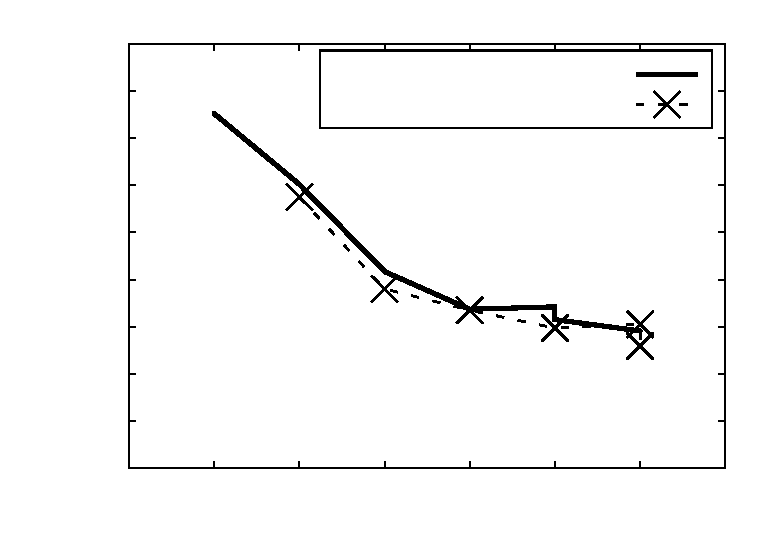
\includegraphics{graphs/scalability/recovery_time_paper}}%
    \gplfronttext
  \end{picture}%
\endgroup
}
      }
  }
  \caption{Recovery time and scalability.}
  \vspace{-3mm}
\end{figure}

We measured the duration of the restrain period considering two clients with a constant throughput of 400 requests/sec. The serial replay mode is not capable of fully exploring the application servers so it takes almost one hour to recover (2953s total, 1100s in restrain mode) (Fig. \ref{fig:restrain:serial}). The clustered mode takes 10 minutes (635s), from which the restrain period represents 46 seconds. (Fig. \ref{fig:restrain:clustered}).
%due to implementation issues

\begin{figure}[tbh]
\vspace{-5mm}
  \LARGE
  \mbox{
    \subfloat[][Serial \label{fig:restrain:serial}]{
      \hspace{-0.5cm}
      \resizebox{4.5cm}{!}{% GNUPLOT: LaTeX picture with Postscript
\begingroup
  \makeatletter
  \providecommand\color[2][]{%
    \GenericError{(gnuplot) \space\space\space\@spaces}{%
      Package color not loaded in conjunction with
      terminal option `colourtext'%
    }{See the gnuplot documentation for explanation.%
    }{Either use 'blacktext' in gnuplot or load the package
      color.sty in LaTeX.}%
    \renewcommand\color[2][]{}%
  }%
  \providecommand\includegraphics[2][]{%
    \GenericError{(gnuplot) \space\space\space\@spaces}{%
      Package graphicx or graphics not loaded%
    }{See the gnuplot documentation for explanation.%
    }{The gnuplot epslatex terminal needs graphicx.sty or graphics.sty.}%
    \renewcommand\includegraphics[2][]{}%
  }%
  \providecommand\rotatebox[2]{#2}%
  \@ifundefined{ifGPcolor}{%
    \newif\ifGPcolor
    \GPcolorfalse
  }{}%
  \@ifundefined{ifGPblacktext}{%
    \newif\ifGPblacktext
    \GPblacktexttrue
  }{}%
  % define a \g@addto@macro without @ in the name:
  \let\gplgaddtomacro\g@addto@macro
  % define empty templates for all commands taking text:
  \gdef\gplbacktext{}%
  \gdef\gplfronttext{}%
  \makeatother
  \ifGPblacktext
    % no textcolor at all
    \def\colorrgb#1{}%
    \def\colorgray#1{}%
  \else
    % gray or color?
    \ifGPcolor
      \def\colorrgb#1{\color[rgb]{#1}}%
      \def\colorgray#1{\color[gray]{#1}}%
      \expandafter\def\csname LTw\endcsname{\color{white}}%
      \expandafter\def\csname LTb\endcsname{\color{black}}%
      \expandafter\def\csname LTa\endcsname{\color{black}}%
      \expandafter\def\csname LT0\endcsname{\color[rgb]{1,0,0}}%
      \expandafter\def\csname LT1\endcsname{\color[rgb]{0,1,0}}%
      \expandafter\def\csname LT2\endcsname{\color[rgb]{0,0,1}}%
      \expandafter\def\csname LT3\endcsname{\color[rgb]{1,0,1}}%
      \expandafter\def\csname LT4\endcsname{\color[rgb]{0,1,1}}%
      \expandafter\def\csname LT5\endcsname{\color[rgb]{1,1,0}}%
      \expandafter\def\csname LT6\endcsname{\color[rgb]{0,0,0}}%
      \expandafter\def\csname LT7\endcsname{\color[rgb]{1,0.3,0}}%
      \expandafter\def\csname LT8\endcsname{\color[rgb]{0.5,0.5,0.5}}%
    \else
      % gray
      \def\colorrgb#1{\color{black}}%
      \def\colorgray#1{\color[gray]{#1}}%
      \expandafter\def\csname LTw\endcsname{\color{white}}%
      \expandafter\def\csname LTb\endcsname{\color{black}}%
      \expandafter\def\csname LTa\endcsname{\color{black}}%
      \expandafter\def\csname LT0\endcsname{\color{black}}%
      \expandafter\def\csname LT1\endcsname{\color{black}}%
      \expandafter\def\csname LT2\endcsname{\color{black}}%
      \expandafter\def\csname LT3\endcsname{\color{black}}%
      \expandafter\def\csname LT4\endcsname{\color{black}}%
      \expandafter\def\csname LT5\endcsname{\color{black}}%
      \expandafter\def\csname LT6\endcsname{\color{black}}%
      \expandafter\def\csname LT7\endcsname{\color{black}}%
      \expandafter\def\csname LT8\endcsname{\color{black}}%
    \fi
  \fi
  \setlength{\unitlength}{0.0500bp}%
  \begin{picture}(7200.00,5040.00)%
    \gplgaddtomacro\gplbacktext{%
      \csname LTb\endcsname%
      \put(1078,704){\makebox(0,0)[r]{\strut{} 0}}%
      \put(1078,1458){\makebox(0,0)[r]{\strut{} 500}}%
      \put(1078,2212){\makebox(0,0)[r]{\strut{} 1000}}%
      \put(1078,2966){\makebox(0,0)[r]{\strut{} 1500}}%
      \put(1078,3720){\makebox(0,0)[r]{\strut{} 2000}}%
      \put(1078,4473){\makebox(0,0)[r]{\strut{} 2500}}%
      \put(1210,484){\makebox(0,0){\strut{}00:00}}%
      \put(2329,484){\makebox(0,0){\strut{}10:00}}%
      \put(3447,484){\makebox(0,0){\strut{}20:00}}%
      \put(4566,484){\makebox(0,0){\strut{}30:00}}%
      \put(5684,484){\makebox(0,0){\strut{}40:00}}%
      \put(6803,484){\makebox(0,0){\strut{}50:00}}%
      \put(176,2739){\rotatebox{-270}{\makebox(0,0){\strut{}Requests per second}}}%
      \put(4006,154){\makebox(0,0){\strut{}Time (minutes:seconds)}}%
      \put(4659,2966){\makebox(0,0)[l]{\strut{}Restrain}}%
    }%
    \gplgaddtomacro\gplfronttext{%
      \csname LTb\endcsname%
      \put(2398,4481){\makebox(0,0)[r]{\strut{}serial}}%
      \csname LTb\endcsname%
      \put(2398,4195){\makebox(0,0)[r]{\strut{}client}}%
    }%
    \gplbacktext
    \put(0,0){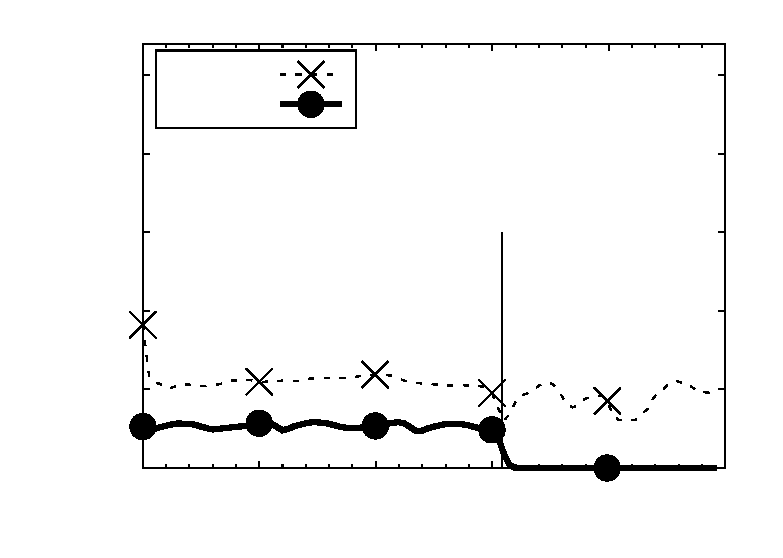
\includegraphics{graphs/restrain/serial_paper}}%
    \gplfronttext
  \end{picture}%
\endgroup
}
    }
    \subfloat[][Clustered \label{fig:restrain:clustered}]{
      \hspace{-0.7cm}
      \resizebox{4.5cm}{!}{% GNUPLOT: LaTeX picture with Postscript
\begingroup
  \makeatletter
  \providecommand\color[2][]{%
    \GenericError{(gnuplot) \space\space\space\@spaces}{%
      Package color not loaded in conjunction with
      terminal option `colourtext'%
    }{See the gnuplot documentation for explanation.%
    }{Either use 'blacktext' in gnuplot or load the package
      color.sty in LaTeX.}%
    \renewcommand\color[2][]{}%
  }%
  \providecommand\includegraphics[2][]{%
    \GenericError{(gnuplot) \space\space\space\@spaces}{%
      Package graphicx or graphics not loaded%
    }{See the gnuplot documentation for explanation.%
    }{The gnuplot epslatex terminal needs graphicx.sty or graphics.sty.}%
    \renewcommand\includegraphics[2][]{}%
  }%
  \providecommand\rotatebox[2]{#2}%
  \@ifundefined{ifGPcolor}{%
    \newif\ifGPcolor
    \GPcolorfalse
  }{}%
  \@ifundefined{ifGPblacktext}{%
    \newif\ifGPblacktext
    \GPblacktexttrue
  }{}%
  % define a \g@addto@macro without @ in the name:
  \let\gplgaddtomacro\g@addto@macro
  % define empty templates for all commands taking text:
  \gdef\gplbacktext{}%
  \gdef\gplfronttext{}%
  \makeatother
  \ifGPblacktext
    % no textcolor at all
    \def\colorrgb#1{}%
    \def\colorgray#1{}%
  \else
    % gray or color?
    \ifGPcolor
      \def\colorrgb#1{\color[rgb]{#1}}%
      \def\colorgray#1{\color[gray]{#1}}%
      \expandafter\def\csname LTw\endcsname{\color{white}}%
      \expandafter\def\csname LTb\endcsname{\color{black}}%
      \expandafter\def\csname LTa\endcsname{\color{black}}%
      \expandafter\def\csname LT0\endcsname{\color[rgb]{1,0,0}}%
      \expandafter\def\csname LT1\endcsname{\color[rgb]{0,1,0}}%
      \expandafter\def\csname LT2\endcsname{\color[rgb]{0,0,1}}%
      \expandafter\def\csname LT3\endcsname{\color[rgb]{1,0,1}}%
      \expandafter\def\csname LT4\endcsname{\color[rgb]{0,1,1}}%
      \expandafter\def\csname LT5\endcsname{\color[rgb]{1,1,0}}%
      \expandafter\def\csname LT6\endcsname{\color[rgb]{0,0,0}}%
      \expandafter\def\csname LT7\endcsname{\color[rgb]{1,0.3,0}}%
      \expandafter\def\csname LT8\endcsname{\color[rgb]{0.5,0.5,0.5}}%
    \else
      % gray
      \def\colorrgb#1{\color{black}}%
      \def\colorgray#1{\color[gray]{#1}}%
      \expandafter\def\csname LTw\endcsname{\color{white}}%
      \expandafter\def\csname LTb\endcsname{\color{black}}%
      \expandafter\def\csname LTa\endcsname{\color{black}}%
      \expandafter\def\csname LT0\endcsname{\color{black}}%
      \expandafter\def\csname LT1\endcsname{\color{black}}%
      \expandafter\def\csname LT2\endcsname{\color{black}}%
      \expandafter\def\csname LT3\endcsname{\color{black}}%
      \expandafter\def\csname LT4\endcsname{\color{black}}%
      \expandafter\def\csname LT5\endcsname{\color{black}}%
      \expandafter\def\csname LT6\endcsname{\color{black}}%
      \expandafter\def\csname LT7\endcsname{\color{black}}%
      \expandafter\def\csname LT8\endcsname{\color{black}}%
    \fi
  \fi
  \setlength{\unitlength}{0.0500bp}%
  \begin{picture}(7200.00,5040.00)%
    \gplgaddtomacro\gplbacktext{%
      \csname LTb\endcsname%
      \put(1078,704){\makebox(0,0)[r]{\strut{} 0}}%
      \put(1078,1458){\makebox(0,0)[r]{\strut{} 500}}%
      \put(1078,2212){\makebox(0,0)[r]{\strut{} 1000}}%
      \put(1078,2966){\makebox(0,0)[r]{\strut{} 1500}}%
      \put(1078,3720){\makebox(0,0)[r]{\strut{} 2000}}%
      \put(1078,4473){\makebox(0,0)[r]{\strut{} 2500}}%
      \put(1210,484){\makebox(0,0){\strut{}00:00}}%
      \put(2795,484){\makebox(0,0){\strut{}03:00}}%
      \put(4381,484){\makebox(0,0){\strut{}06:00}}%
      \put(5966,484){\makebox(0,0){\strut{}09:00}}%
      \put(176,2739){\rotatebox{-270}{\makebox(0,0){\strut{}Requests per second}}}%
      \put(4006,154){\makebox(0,0){\strut{}Time (minutes:seconds)}}%
      \put(5174,4473){\makebox(0,0)[l]{\strut{}Restrain}}%
    }%
    \gplgaddtomacro\gplfronttext{%
      \csname LTb\endcsname%
      \put(2794,4481){\makebox(0,0)[r]{\strut{}clustered}}%
      \csname LTb\endcsname%
      \put(2794,4195){\makebox(0,0)[r]{\strut{}client}}%
    }%
    \gplbacktext
    \put(0,0){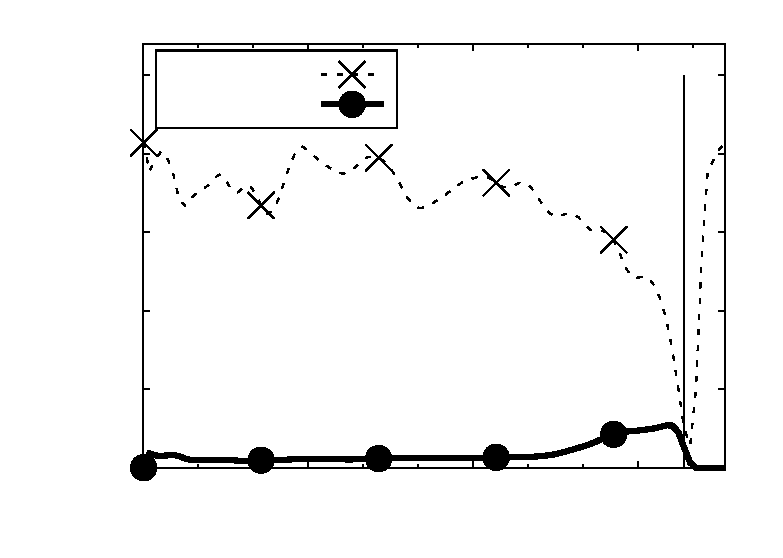
\includegraphics{graphs/restrain/clustered_paper}}%
    \gplfronttext
  \end{picture}%
\endgroup
}
    }
  }
  \caption{Restrain period in serial and clustered recovery (\emph{Restrain} indicates the beggining of the period that ends at the end of the graphic).}
  \vspace{-3mm}
\end{figure}


\textbf{Space overhead.}
%Shuttle implies a fixed network overhead for attaching a \acf{SRD} (35 bytes) to every request and database access.
We measured the memory and storage overhead of 1 million requests, from which 95\% were requests for reading questions. Table \ref{tab:storage_overhead} presents the size of each component in memory\LONG{footnote{https://code.google.com/p/memory-measurer}}. Requests and keys are stored in the external database while the dependency graph and the accesses are kept in the manager and database instances. No snapshot has been taken and the data is not compressed.
%
In the current implementation, the \ac{SRD} represents a fixed overhead of 35 bytes per request.

\begin{table}[h]
\centering
\footnotesize
  \begin{tabular}{l|rr}
                & \# objects & size (MB) \\ \hline
  \textbf{Shuttle Storage: }      \\
  Request         & 1 million    & 212       \\  %1000000 - 212 162 883  old: & 200314    & 41,5 \\
  Response        & 1 million    & 8 967     \\  %1000000 - 8 967 233 474 old & 200314    & 1954 \\
  Start/end timestamps      & 2 million    & 16        \\  %2000000 - 16 000 000   old: & 200314    & 3,2  \\
  Keys            & 137 million  & 488       \\  %137 244 585  - 488 862 483 old: & 200314    & 105,2\\
  Total           &              & 9 684     \\  %9 684258 840
  \textbf{Database node:}        &           \\
  Version List    &  14 593      &  1.4       \\ %14 593 - 1 400 928   - 96 bytes old: & 3079     & 27,9 \\
  Operation list  &  9 million   &  277       \\ %9 551 908 - 277 019 984   - 29 bytes old: &  2061521  & 9,65 \\
  Total           &              & 282 \\ %282 230 960   old: & 61,3 \\
  \textbf{Manager:} & & \\ 
  Graph           & 1 million    & 718 \\  %718 486 432 old: & 200314    & 153,2 \\
  \end{tabular}            
\caption{Storage used by Shuttle  (1 million requests).}
\label{tab:storage_overhead}
\vspace{-5mm}
\end{table}

The main overhead are the responses, as we are storing them complete (full HTML pages), although  Shuttle has to store them only if the tenant uses the API to solve inconsistencies (Section \ref{sec:recovery:consistency}). The size of the list of keys accessed by the request depends on the key length and the number of keys accessed. Each access implies an overhead of 13 bytes to record the request ID and the operation type in the version list. The snapshot does not impact the throughput but requires to track the new version, which implies a storage overhead of 10 bytes for each data item when it is written by the first time after a snapshot. This overhead can be reduced implementing the version list as a bitmap. The total database storage overhead encompasses synchronization mechanisms. Since the dependency graph is implemented as a double-linked graph, each entry in the dependency graph has 765 bytes to store not only the start/end instant of the request but also the requests which this request depends from and to (10 on average). Serialization mechanisms and compression techniques can reduce the storage overhead. For instance, Cassandra's \emph{lz4}\LONG{cite{lz4}} reduces the size of the Shuttle Storage on disk to 4.9 GB.

%For the sake of simplicity, the dependency graph is doubly-linked, a single-linked graph requires 458 bytes per entry. 

\textbf{Monetary cost.}
%\label{sec:evaluation:cost}
%
Since the replay instances are allocated on demand and paid per use, the cost of Shuttle is dominated by the storage. 
For instance, consider the extreme case of 20 million requests/day with overhead proportional to the values in Table \ref{tab:storage_overhead} to show that the costs are not high. To store it Shuttle would need 1.432 TB in Shuttle Storage, 1.436 TB for the graph and 564 GB in the database. 
To reduce this cost in AWS, we could combine DynamoDB with Glacier, a high latency / low cost storage service. Shuttle might store the last 24 hours of requests on DynamoDB and the rest on Glacier. In this scenario, Shuttle generates 35 GB per day (except the responses), which costs \$8.75 per month to store in DynamoDB and \$4.83 per-month for the provisioned capacity. Glacier would store 3.433 TB with a cost of \$34.33 per month. Since Shuttle performs snapshots, tenants can remove old snapshots tacking into account that Shuttle needs only a snapshot previous to the intrusion instant to recover the application.

Shuttle requires an extra instance to deploy the Shuttle manager. To recover the application, we used one \emph{c3.xlarge} virtual machine as replay instance and two  \emph{c3.xlarge} instances to run the application servers to replay 1 million requests during 544 seconds. Considering a full-hour, these instances have a cost of \$0.239 per instance-hour, which means a cost of less than \$1 for the recovery. In this manner, Shuttle leverages the elasticity and pay-per-usage model of cloud computing to provide a cost-efficient intrusion recovery solution.

%%!TEX root = ../paper.tex
%!TEX encoding = UTF-8 Unicode

\section{Related Work}
\label{sec:related_work}

Shuttle is an intrusion recovery system based on log replay. While this approach has been applied in operating systems \cite{taser,retro,dare}, databases \cite{itdb,phoenix}, and web services \cite{warp,goel,aire}, our system is the only one that recovers from intrusions in applications deployed on \ac{PaaS} platforms with multiple servers. The closest works to Shuttle are Aire \cite{aire}, Warp \cite{warp}, Goel \cite{goel}, and Undo for Operators (UO) \cite{undoForOperators}, although none of them does recovery in cloud environments.

Shuttle's full replay approach is motivated by UO \cite{undoForOperators}. UO removes the intrusion effects using a snapshot and replaying every request after the snapshot instant.\LONG{However, the primary source of difference between the two approaches is their target applications.} UO considers monolithic applications, which are instantiated in the paper as an email server. Shuttle, on the contrary, considers a \ac{PaaS} platform with both application server and database instances, supporting scalable applications of several kinds\LONG{(e.g., Q\&A, social networks, shared editors, etc.)}. UO sorts requests using knowledge of the application protocol. Developers must define, for each type of application request, the order between requests and their capability to be executed in parallel. In contrast, Shuttle uses the dependency graph to create clusters of request to execute in parallel and sorts the requests using the start-end order and database accesses.

%mpc: cuidado: nao e' et. all mas et al. (abreviatura de "et alia")

Goel \emph{et al.} \cite{goel} proposes a solution to recover from intrusion in web applications. It uses a modified PHP interpreter to determine the tainted requests. Goel reverts the effect of tainted requests applying compensating transactions on the current state of the database. %Unlike Shuttle, it does not replay requests. Therefore, effects of legitimate actions, which have been tainted, are lost.

Warp \cite{warp} helps the administrators to retroactively patch security vulnerabilities. It stores every version of each data item and the version read by each request. It also captures the browser-side input at DOM level using a browser plugin and modifies the code interpreter to track the code files invoked by each request. Requests that invoked code files modified by the patch are considered tainted. Warp loads the version of the tainted data items and repeats these requests using a server-side browser. Forward requests are also replayed while their inputs are different from the ones at first execution. Most of previous solutions store every data item version or action input and output \cite{warp,aire}. Shuttle incurs on smaller storage overhead because it gets the data item version from a snapshot and replays every legitimate request at least until the next snapshot, where the data item value is known.

%Get previous values
There have been different approaches to remove the intrusion effects: Goel \emph{et al.} use transaction compensation to create a snapshot, Warp stores every data item version and UO uses snapshots. While the first does not remove the effects of unknown actions, the second requires a considerable storage overhead. We implemented a snapshot mechanism designed for distributed databases. While UO overwrites the current state copying an old snapshot, we use the \textit{branch path} mechanism to select the accessible snapshots for a given request without copying data.

%runtime recovery:
Warp supports recovery in runtime using two fields in the database table, whereas Aire uses a branching mechanism to permit recovery on loosely coupled web services. We use a branching mechanism to support runtime recovery allowing various recovery processes simultaneously. 

%inconsistency
Goel \emph{et al.} does not address external consistency issues. Warp \cite{warp} detects inconsistencies in responses and replays the user interaction using a browser. UO uses compensating actions based on protocol-specific knowledge. We propose an API that the application developers can use to deal with inconsistencies.


%!TEX root = ../tese.tex
%!TEX encoding = UTF-8 Unicode
\chapter{Conclusion}\label{chapter:conclusion}
This dissertation described Shuttle, the first intrusion recovery system for \acf{PaaS} that uses a record-and-replay approach. We aim to define a generic architecture that allows \acf{CSP} to offer an intrusion recovery system as a service to their tenants. This service is available without setup and can be provided in a pay-per-usage manner. Our research focused on developing a scalable service to meet the intrusion recovery of Cloud tenants. The success of Shuttle will be measured mostly by the impact of two of this dissertation's main contributions: a service integrated in \ac{PaaS} that leverages the resource elasticity and pay-per-use model and a new process to establish the requests' order during the replay process.

This chapter reflects on these contributions, discusses future work and concludes.

\section{Conclusions}\label{sec:conclusion:conclusion}
%Contributions to related work
Our approach to develop an intrusion recovery system for cloud computing focus on restoring the applications integrity when intrusions happen, instead of trying to prevent them from happening. Previous works address this problem at operating system level \cite{taser,retro} or distributed systems \cite{aire}. These systems might be adapted to recover from intrusions in the \acf{IaaS} model. Other works aim to recover databases \cite{itdb,phoenix} and web services \cite{warp,goel,aire}, so they can be adapted to recover services delivered in the \acf{SaaS} model. The closest research to ours is Undo for Operators (UO) \cite{undoForOperators}. Both works address the problem of providing a generic intrusion recovery system. However, UO requires tenants to configure the dependencies and order for each possible operation of the application's protocol. Our approach does not require configuration. Nevertheless, none of the previous works does recovery in cloud environments. We consider an intrusion recovery system to be a significant asset for CSPs because they are responsible for managing the \ac{PaaS} applications and ensure their security. The \ac{PaaS} model imposes novel challenges because its applications scale and run in various instances backed by distributed databases. \\

Having the above in mind, we proposed Shuttle, an intrusion recovery service for \ac{PaaS}, that aims to make \ac{PaaS} applications operational despite intrusions. Shuttle recovers from software flaws and corrupted requests. As consequence of its architecture, our solution also supports preventive maintenance and to test the application with real user requests. Shuttle loads database snapshots to remove the intrusion effects and replays the legitimate user requests to recover the application integrity.

%Remove
In order to remove the intrusion effects, we proposed a novel method to perform snapshots of \acs{NoSQL} databases. This method, which is based on copy-on-write, performs globally transaction-consistent and incremental snapshots without system downtime. We also proposed a novel process that redeploys tenants' application in new application instances to remove all intrusions in the previous instances and update their software versions to fix previous flaws or prevent future vulnerability exploitations.\\

%Restore
In order to restore the application integrity, we proposed a new method to re-execute requests. This method supports that the requests have been executed concurrently. It replays the requests on the same order than on their first execution and constrains the execution order using the list of operations performed on each database item. Since database items are independent, our replay algorithm is scalable. In addition, we proposed a semantic-reconciliation mechanism to solve conflicts during the recovery process.

Previous works use the dependency graph to establish the requests order. Instead, we use it to create independent clusters of requests that can be re-executed concurrently. We evaluated that this technique reduces the recovery period considerably.

We accomplish intrusion recovery without service downtime using a branching mechanism.

In summary, the proposed architecture is capable of leveraging the resource elasticity and pay-per-use model in \ac{PaaS} environments to record and launch multiple clients to replay previous non-malicious user requests as concurrently as possible to reduce the recovery time and costs.

Thus, we have achieved the goal we set out at the beginning of this dissertation: help \acf{CSP} customers to recover from intrusions in their applications deployed in \acf{PaaS}.

\section{Future Work}\label{sec:conclusion:future_work}
The following directions are proposed as a development of the present research:
\begin{itemize}
\item Consider the dependencies and result on client's browser: a considerable trend in web-application development is moving the application code to the client's browser. How this will affect the dependencies between requests? How will be the consistency of the replay process?
\item Consider more database schemas and operations operations: several operations such as \emph{scan} and \emph{append}. What applications can be build using idempotent operations? How the replay algorithms can encompass them?
\item Consider the user sessions in the dependency algorithms.
\item Fault-tolerance: how to handle when the recovery process fails when instances fail \hl{quando as instancias, por exemplo de replay, falham}? How to handle database replication?
\item Research about how the instance rejuvenation can be used in \ac{PaaS} to prevent attackers from compromise a quorum of replicas.
\item Extend the evaluation scenarios tests to more complex intrusions.
\item Evaluate the dependencies created by several types of applications.
\item Propose mechanisms to prevent intrusions from spreading.
\item Propose a pricing model to deliver a intrusion recovery system on a pay-per-usage manner.
\end{itemize}


\hl{Exacto, há aqui ideias que são apenas prolongamentos ou requisitos para colocar em producao. Queria falar consigo para seleccionarmos apenas 80\% delas no máximo. }
In addition, we propose to develop an user interface for tenants and evaluate their experience. A distinct research direction can evaluate how intrusion recover system for cloud, such as Shuttle, can be integrated and affect the recovery procedures of companies. In particular, how these systems can be integrated and used by the practices, for instance, defined in the Service Design and Service Operation aspects of \ac{ITIL}. By doing so, we expect to analyze the advantages and disadvantages of using these services.

The major challenges to implement the current prototype were: concurrent and consistent database snapshot, establish accurate requests dependencies, perform parallel actions replay, repair the system state in time, avoid application downtime and keep the application source code unmodified as much as possible.

As future work, we would like to improve the implementation by:
\begin{itemize}
\item Optimize the concurrency mechanisms serial replay in the replay instances
\item Migrate the dependency graph to a distributed database
\item Improve the clustering algorithm
\item Integrate the proxy in a load-balancer implementation
\item Analyze compression mechanisms to reduce the memory and storage footprint
\end{itemize}


Shuttle removes intrusions' effects in \ac{PaaS} applications and restores their state to an intrusion-free state. We propose, to the best of our knowledge, the first intrusion recovery service for \ac{PaaS} and the first to support \acs{NoSQL} databases.


%-------------------------------------------------------------------------
%\appendix
%\section{Appendix Title}
%This is the text of the appendix, if you need one.

% \acks
% This work was supported by INESC-ID - Distributed Systems group and part of RC-Clouds - Resilient Computing in Clouds - research project funded by FCT- Fundação para a Ciência e a Tecnologia (PTDC/EIA-EIA/115211/2009). 

%ACM: \bibliographystyle{abbrvnat}
\bibliographystyle{IEEEtran}

{\footnotesize
\bibliography{refs/ALL.bib,refs/manual.bib}
}
%\begin{thebibliography}{}
%\softraggedright
%\bibitem[Smith et~al.(2009)Smith, Jones]{smith02}
%P. Q. Smith, and X. Y. Jones. ...reference text...
%\end{thebibliography}


\end{document}




